\documentclass[8pt,ignorenonframetext,dvipsnames]{beamer}
\setbeamertemplate{caption}[numbered]
\setbeamertemplate{caption label separator}{: }
\setbeamercolor{caption name}{fg=normal text.fg}
\beamertemplatenavigationsymbolsempty
\usepackage{lmodern}
\usepackage{amssymb,amsmath}
\usepackage{ifxetex,ifluatex}
\usepackage{fixltx2e} % provides \textsubscript
\ifnum 0\ifxetex 1\fi\ifluatex 1\fi=0 % if pdftex
  \usepackage[T1]{fontenc}
  \usepackage[utf8]{inputenc}
\else % if luatex or xelatex
  \ifxetex
    \usepackage{mathspec}
  \else
    \usepackage{fontspec}
  \fi
  \defaultfontfeatures{Ligatures=TeX,Scale=MatchLowercase}
\fi
% use upquote if available, for straight quotes in verbatim environments
\IfFileExists{upquote.sty}{\usepackage{upquote}}{}
% use microtype if available
\IfFileExists{microtype.sty}{%
\usepackage{microtype}
\UseMicrotypeSet[protrusion]{basicmath} % disable protrusion for tt fonts
}{}
\newif\ifbibliography
\hypersetup{
            pdftitle={Lecture 2: Investigating data patterns},
            pdfauthor={Ozan Jaquette},
            colorlinks=true,
            linkcolor=Maroon,
            citecolor=Blue,
            urlcolor=blue,
            breaklinks=true}
\urlstyle{same}  % don't use monospace font for urls
\usepackage{color}
\usepackage{fancyvrb}
\newcommand{\VerbBar}{|}
\newcommand{\VERB}{\Verb[commandchars=\\\{\}]}
\DefineVerbatimEnvironment{Highlighting}{Verbatim}{commandchars=\\\{\}}
% Add ',fontsize=\small' for more characters per line
\usepackage{framed}
\definecolor{shadecolor}{RGB}{248,248,248}
\newenvironment{Shaded}{\begin{snugshade}}{\end{snugshade}}
\newcommand{\KeywordTok}[1]{\textcolor[rgb]{0.13,0.29,0.53}{\textbf{#1}}}
\newcommand{\DataTypeTok}[1]{\textcolor[rgb]{0.13,0.29,0.53}{#1}}
\newcommand{\DecValTok}[1]{\textcolor[rgb]{0.00,0.00,0.81}{#1}}
\newcommand{\BaseNTok}[1]{\textcolor[rgb]{0.00,0.00,0.81}{#1}}
\newcommand{\FloatTok}[1]{\textcolor[rgb]{0.00,0.00,0.81}{#1}}
\newcommand{\ConstantTok}[1]{\textcolor[rgb]{0.00,0.00,0.00}{#1}}
\newcommand{\CharTok}[1]{\textcolor[rgb]{0.31,0.60,0.02}{#1}}
\newcommand{\SpecialCharTok}[1]{\textcolor[rgb]{0.00,0.00,0.00}{#1}}
\newcommand{\StringTok}[1]{\textcolor[rgb]{0.31,0.60,0.02}{#1}}
\newcommand{\VerbatimStringTok}[1]{\textcolor[rgb]{0.31,0.60,0.02}{#1}}
\newcommand{\SpecialStringTok}[1]{\textcolor[rgb]{0.31,0.60,0.02}{#1}}
\newcommand{\ImportTok}[1]{#1}
\newcommand{\CommentTok}[1]{\textcolor[rgb]{0.56,0.35,0.01}{\textit{#1}}}
\newcommand{\DocumentationTok}[1]{\textcolor[rgb]{0.56,0.35,0.01}{\textbf{\textit{#1}}}}
\newcommand{\AnnotationTok}[1]{\textcolor[rgb]{0.56,0.35,0.01}{\textbf{\textit{#1}}}}
\newcommand{\CommentVarTok}[1]{\textcolor[rgb]{0.56,0.35,0.01}{\textbf{\textit{#1}}}}
\newcommand{\OtherTok}[1]{\textcolor[rgb]{0.56,0.35,0.01}{#1}}
\newcommand{\FunctionTok}[1]{\textcolor[rgb]{0.00,0.00,0.00}{#1}}
\newcommand{\VariableTok}[1]{\textcolor[rgb]{0.00,0.00,0.00}{#1}}
\newcommand{\ControlFlowTok}[1]{\textcolor[rgb]{0.13,0.29,0.53}{\textbf{#1}}}
\newcommand{\OperatorTok}[1]{\textcolor[rgb]{0.81,0.36,0.00}{\textbf{#1}}}
\newcommand{\BuiltInTok}[1]{#1}
\newcommand{\ExtensionTok}[1]{#1}
\newcommand{\PreprocessorTok}[1]{\textcolor[rgb]{0.56,0.35,0.01}{\textit{#1}}}
\newcommand{\AttributeTok}[1]{\textcolor[rgb]{0.77,0.63,0.00}{#1}}
\newcommand{\RegionMarkerTok}[1]{#1}
\newcommand{\InformationTok}[1]{\textcolor[rgb]{0.56,0.35,0.01}{\textbf{\textit{#1}}}}
\newcommand{\WarningTok}[1]{\textcolor[rgb]{0.56,0.35,0.01}{\textbf{\textit{#1}}}}
\newcommand{\AlertTok}[1]{\textcolor[rgb]{0.94,0.16,0.16}{#1}}
\newcommand{\ErrorTok}[1]{\textcolor[rgb]{0.64,0.00,0.00}{\textbf{#1}}}
\newcommand{\NormalTok}[1]{#1}
\usepackage{longtable,booktabs}
\usepackage{caption}
% These lines are needed to make table captions work with longtable:
\makeatletter
\def\fnum@table{\tablename~\thetable}
\makeatother
\usepackage{graphicx,grffile}
\makeatletter
\def\maxwidth{\ifdim\Gin@nat@width>\linewidth\linewidth\else\Gin@nat@width\fi}
\def\maxheight{\ifdim\Gin@nat@height>\textheight0.8\textheight\else\Gin@nat@height\fi}
\makeatother
% Scale images if necessary, so that they will not overflow the page
% margins by default, and it is still possible to overwrite the defaults
% using explicit options in \includegraphics[width, height, ...]{}
\setkeys{Gin}{width=\maxwidth,height=\maxheight,keepaspectratio}

% Prevent slide breaks in the middle of a paragraph:
\widowpenalties 1 10000
\raggedbottom

\AtBeginPart{
  \let\insertpartnumber\relax
  \let\partname\relax
  \frame{\partpage}
}
\AtBeginSection{
  \ifbibliography
  \else
    \let\insertsectionnumber\relax
    \let\sectionname\relax
    \frame{\sectionpage}
  \fi
}
\AtBeginSubsection{
  \let\insertsubsectionnumber\relax
  \let\subsectionname\relax
  \frame{\subsectionpage}
}

\setlength{\parindent}{0pt}
\setlength{\parskip}{6pt plus 2pt minus 1pt}
\setlength{\emergencystretch}{3em}  % prevent overfull lines
\providecommand{\tightlist}{%
  \setlength{\itemsep}{0pt}\setlength{\parskip}{0pt}}
\setcounter{secnumdepth}{0}

%packages
\usepackage{graphicx}
\usepackage{rotating}
\usepackage{hyperref}

\usepackage{tikz} % used for text highlighting, amongst others
%title slide stuff
%\institute{Department of Education}
%\title{Managing and Manipulating Data Using R}

%
\setbeamertemplate{navigation symbols}{} % get rid of navigation icons:

%\setbeamertemplate{frametitle}{\thesection \hspace{0.2cm} \insertframetitle}
\setbeamertemplate{section in toc}[sections numbered]
%\setbeamertemplate{subsection in toc}[subsections numbered]
\setbeamertemplate{subsection in toc}{%
  \leavevmode\leftskip=3.2em\color{gray}\rlap{\hskip-2em\inserttocsectionnumber.\inserttocsubsectionnumber}\inserttocsubsection\par
}

%define colors
%\definecolor{uva_orange}{RGB}{216,141,42} % UVa orange (Rotunda orange)
\definecolor{mygray}{rgb}{0.95, 0.95, 0.95} % for highlighted text
	% grey is equal parts red, green, blue. higher values >> lighter grey
	%\definecolor{lightgraybo}{rgb}{0.83, 0.83, 0.83}

% new commands

%highlight text with very light grey
\newcommand*{\hlg}[1]{%
	\tikz[baseline=(X.base)] \node[rectangle, fill=mygray] (X) {#1};%
}
%, inner sep=0.3mm
%highlight text with very light grey and use font associated with code
\newcommand*{\hlgc}[1]{\texttt{\hlg{#1}}}

% Font
\usepackage[defaultfam,light,tabular,lining]{montserrat}
\usepackage[T1]{fontenc}
\renewcommand*\oldstylenums[1]{{\fontfamily{Montserrat-TOsF}\selectfont #1}}

% Change color of boldface text to darkgray
\renewcommand{\textbf}[1]{{\color{darkgray}\bfseries\fontfamily{Montserrat-TOsF}#1}}

% Bullet points
\setbeamertemplate{itemize item}{\color{BlueViolet}$\circ$}
\setbeamertemplate{itemize subitem}{\color{BrickRed}$\triangleright$}
\setbeamertemplate{itemize subsubitem}{$-$}

% Reduce space before lists
\addtobeamertemplate{itemize/enumerate body begin}{}{\vspace*{-8pt}}

\let\olditem\item
\renewcommand{\item}{%
  \olditem\vspace{4pt}
}

% decreasing space before and after level-2 bullet block
\addtobeamertemplate{itemize/enumerate subbody begin}{}{\vspace*{-3pt}}
\addtobeamertemplate{itemize/enumerate subbody end}{}{\vspace*{-3pt}}

% decreasing space before and after level-3 bullet block
\addtobeamertemplate{itemize/enumerate subsubbody begin}{}{\vspace*{-2pt}}
\addtobeamertemplate{itemize/enumerate subsubbody end}{}{\vspace*{-2pt}}

%Section numbering
\setbeamertemplate{section page}{%
    \begingroup
        \begin{beamercolorbox}[sep=10pt,center,rounded=true,shadow=true]{section title}
        \usebeamerfont{section title}\thesection~\insertsection\par
        \end{beamercolorbox}
    \endgroup
}

\setbeamertemplate{subsection page}{%
    \begingroup
        \begin{beamercolorbox}[sep=6pt,center,rounded=true,shadow=true]{subsection title}
        \usebeamerfont{subsection title}\thesection.\thesubsection~\insertsubsection\par
        \end{beamercolorbox}
    \endgroup
}

%modifying back ticks to add grey background
\let\OldTexttt\texttt
\renewcommand{\texttt}[1]{\OldTexttt{\hlg{#1}}}

\title{Lecture 2: Investigating data patterns}
\subtitle{EDUC 263: Managing and Manipulating Data Using R}
\author{Ozan Jaquette}
\date{}

\begin{document}
\frame{\titlepage}

\section{Introduction}\label{introduction}

\begin{frame}{What we will do today}

\tableofcontents

\end{frame}

\begin{frame}[fragile]{Libraries we will use today}

``Load'' the package we will use today (output omitted)

\begin{Shaded}
\begin{Highlighting}[]
\KeywordTok{library}\NormalTok{(tidyverse)}
\end{Highlighting}
\end{Shaded}

If package not yet installed, then must install before you load. Install
in ``console'' rather than .Rmd file

\begin{itemize}
\tightlist
\item
  Generic syntax: \texttt{install.packages("package\_name")}
\item
  Install ``tidyverse'': \texttt{install.packages("tidyverse")}
\end{itemize}

Note: when we load package, name of package is not in quotes; but when
we install package, name of package is in quotes:

\begin{itemize}
\tightlist
\item
  \texttt{install.packages("tidyverse")}
\item
  \texttt{library(tidyverse)}
\end{itemize}

\end{frame}

\section{R Markdown}\label{r-markdown}

\begin{frame}[fragile]{What is R Markdown}

Borrowing from Darin Christensen:

\begin{itemize}
\tightlist
\item
  R Markdown documents embed R code, the output associated with R code,
  and text into one document
\item
  An R Markdown document is a ``\,`Living' document that updates every
  time you compile {[}``knit''{]} it''
\item
  R Markdown documents have the extension .Rmd

  \begin{itemize}
  \tightlist
  \item
    can think of them as text files with the extension .Rmd rather than
    .txt
  \end{itemize}
\item
  At top of .Rmd file you specify the ``output'' style, which dictates
  what kind of formatted document will be created
\item
  When you compile {[}``knit''{]} a .Rmd file, the resulting formatted
  document can be an HTML document, a PDF document, an MS Word document,
  or many other types
\end{itemize}

How we will be using R Markdown files in this class:

\begin{itemize}
\tightlist
\item
  homework you submit will be .Rmd files, with ``output'' style will be
  \texttt{html\_document} or \texttt{pdf\_document}
\item
  lectures we write are .Rmd files, where we the output style will
  usually be \texttt{beamer\_presentation}

  \begin{itemize}
  \tightlist
  \item
    this is essentially a pdf document, where each page is a slide
  \end{itemize}
\end{itemize}

\end{frame}

\begin{frame}[fragile]{Creating RMarkdown documents}

\textbf{Do this with a partner}

Approach for creating a RMarkdown document.

\begin{enumerate}
\def\labelenumi{\arabic{enumi}.}
\tightlist
\item
  Point-and-click from within RStudio

  \begin{itemize}
  \tightlist
  \item
    Click on \emph{File} \textgreater{}\textgreater{} \emph{New File}
    \textgreater{}\textgreater{} \emph{R Markdown}
    \textgreater{}\textgreater{} \emph{Document}
    \textgreater{}\textgreater{} choose \emph{HTML}
    \textgreater{}\textgreater{} click \emph{OK}
  \item
    save the .Rmd file {[}any name, anywhere you can find it{]}
  \item
    ``Knit'' the entire .Rmd file

    \begin{itemize}
    \tightlist
    \item
      point-and-click OR shortcut: \textbf{Cmd/Ctrl + Shift + k}
    \end{itemize}
  \end{itemize}
\end{enumerate}

\begin{Shaded}
\begin{Highlighting}[]
\CommentTok{# 2. From blank text file}
\CommentTok{#     - create blank text file}
\CommentTok{#         - can give it any name, but change extension from .txt to .Rmd}
\CommentTok{#     - Open this blank .Rmd file in Rstudio}
\CommentTok{#     - copy this text into file [LINK HERE][PATRICIA CREATE LINK TO sample_simple_rmarkdown.txt FILE WHICH IS STORED IN LECTURE 2 DIRECTORY]}
\CommentTok{#     - "knit" the entire .Rmd file}
\CommentTok{#         - point-and-click OR shortcut: __Cmd/Ctrl + Shift + k__}

\CommentTok{#Don't worry about this. Ozan's notes}
\end{Highlighting}
\end{Shaded}

\end{frame}

\begin{frame}[fragile]{Components of a .Rmd file}

An RMarkdown (.Rmd) file consists of several parts

\begin{enumerate}
\def\labelenumi{\arabic{enumi}.}
\tightlist
\item
  \textbf{YAML header}

  \begin{itemize}
  \tightlist
  \item
    YAML stands for ``yet another markup language''
  \item
    controls settings that apply to the whole document (e.g., ``output''
    should be html\_document or pdf\_document, whether to include table
    of contents, etc.)
  \item
    YAML header goes at very top of document
  \item
    starts with a line of three horizontal dashes \texttt{-\/-\/-}; ends
    with a line of three horizontal dashes \texttt{-\/-\/-}
  \end{itemize}
\item
  \textbf{Text} in body of .Rmd file

  \begin{itemize}
  \tightlist
  \item
    e.g., headings; description of results, etc.
  \end{itemize}
\item
  \textbf{R code chunks} in body of .Rmd file
\end{enumerate}

\begin{Shaded}
\begin{Highlighting}[]
\NormalTok{a <-}\StringTok{ }\KeywordTok{c}\NormalTok{(}\DecValTok{2}\NormalTok{,}\DecValTok{4}\NormalTok{,}\DecValTok{6}\NormalTok{)}
\NormalTok{a}
\NormalTok{a}\OperatorTok{-}\DecValTok{1}
\end{Highlighting}
\end{Shaded}

\begin{enumerate}
\def\labelenumi{\arabic{enumi}.}
\setcounter{enumi}{3}
\tightlist
\item
  \textbf{R output} associated with code chunks
\end{enumerate}

\begin{verbatim}
#> [1] 2 4 6
#> [1] 1 3 5
\end{verbatim}

\end{frame}

\begin{frame}{Comment: Running R code chunks vs. ``knit'' entire .Rmd
file}

Two ways to execute R commands in .Rmd file:

\begin{enumerate}
\def\labelenumi{\arabic{enumi}.}
\tightlist
\item
  ``Knit'' entire .Rmd file

  \begin{itemize}
  \tightlist
  \item
    shortcut: \textbf{Cmd/Ctrl + Shift + k}
  \end{itemize}
\item
  ``Run'' code chunk or selected lines within code chunk

  \begin{itemize}
  \tightlist
  \item
    Run selected line(s): \textbf{Cmd/Ctrl + Enter}
  \item
    Run current chunk: \textbf{Cmd/Ctrl + Shift + Enter}
  \end{itemize}
\end{enumerate}

Comment on default settings for RStudio:

\begin{itemize}
\tightlist
\item
  When you knit entire .Rmd file, ``objects'' created within .Rmd file
  will not be available after file comples
\item
  When you run code chunk (or selected lines in chunk), objects created
  by lines you run will be in your ``environment'' until you remove them
  or quit R session
\end{itemize}

\end{frame}

\begin{frame}[fragile]{Output types of .Rmd file}

Common/important output types:

\begin{itemize}
\tightlist
\item
  \textbf{html\_document}: R Markdown originally designed to create HTML
  documents

  \begin{itemize}
  \tightlist
  \item
    Most features/code in .Rmd files were written for html\_document
  \item
    many of these features are available in other output types
  \item
    When learning R Markdown, best to start by learning html\_document
  \end{itemize}
\item
  \textbf{pdf\_document}: Requires installation of LaTeX (MiKTeX/MacTeX)

  \begin{itemize}
  \tightlist
  \item
    How it works:

    \begin{itemize}
    \tightlist
    \item
      You write .Rmd code;
    \item
      When you compile, this .Rmd code is transformed into LaTeX code
    \item
      LaTeX ``engine'' creates the formatted .pdf file
    \end{itemize}
  \item
    Can include some of the same features available for
    \emph{html\_document}
  \item
    Can insert LaTeX commands in .Rmd file with \emph{pdf\_document}
    output
  \end{itemize}
\item
  \textbf{beamer\_presentation}: Requires installation of LaTeX

  \begin{itemize}
  \tightlist
  \item
    ``beamer'' is the name for presentations written in LaTeX
  \item
    essentially creates PDF of presentation slides
  \item
    Lectures for this class created with \emph{beamer\_presentation}
    output
  \item
    note: YAML header includes \texttt{beamer\_header.tex} file, which
    creates some formatting rules and additional commands
  \end{itemize}
\end{itemize}

\end{frame}

\begin{frame}{Learning more about R Markdown}

Resources

\begin{itemize}
\tightlist
\item
  Cheat sheets and quick reference:

  \begin{itemize}
  \tightlist
  \item
    \href{https://www.rstudio.com/wp-content/uploads/2015/02/rmarkdown-cheatsheet.pdf}{Cheat
    Sheet}
  \item
    \href{https://www.rstudio.com/wp-content/uploads/2015/03/rmarkdown-reference.pdf}{Quick
    Reference} {[}I prefer the quick reference{]}
  \end{itemize}
\item
  Chapters/books

  \begin{itemize}
  \tightlist
  \item
    \href{http://r4ds.had.co.nz/r-markdown.html}{Chapter 27} of ``R for
    Data Science'' book
  \item
    \href{https://bookdown.org/yihui/rmarkdown/}{R Markdown: The
    Definative Guide} book {[}I prefer this book{]}
  \end{itemize}
\end{itemize}

How you will learn R Markdown

\begin{itemize}
\tightlist
\item
  Lectures written as .Rmd file

  \begin{itemize}
  \tightlist
  \item
    During class run ``code chunks'' and try to ``knit'' entire .Rmd
    file
  \end{itemize}
\item
  I'll assign \textbf{small} amount of reading on R Markdown

  \begin{itemize}
  \tightlist
  \item
    prior to next week:

    \begin{itemize}
    \tightlist
    \item
      spend 10-15 minutes familiarizing yourself with
      \href{https://www.rstudio.com/wp-content/uploads/2015/03/rmarkdown-reference.pdf}{Quick
      Reference}
    \item
      Read section
      \href{https://bookdown.org/yihui/rmarkdown/html-document.html}{3.1
      of R Markdown: The Definative Guide}, about creating
      html\_document
    \end{itemize}
  \end{itemize}
\item
  Homework must be written in .Rmd file

  \begin{itemize}
  \tightlist
  \item
    you submit .Rmd file AND output of compiled file
  \item
    for next week, you will submit homework as html\_document output
  \end{itemize}
\end{itemize}

\end{frame}

\section{More R basics: functions and
directories}\label{more-r-basics-functions-and-directories}

\subsection{Introduction to using
functions}\label{introduction-to-using-functions}

\begin{frame}[fragile]{What are functions}

\medskip \textbf{Functions} are pre-written bits of code that accomplish
some task.

\medskip Functions generally follow three sequential steps:

\begin{enumerate}
\def\labelenumi{\arabic{enumi}.}
\tightlist
\item
  take in an \textbf{input} object(s)
\item
  \textbf{process} the input.
\item
  \textbf{return} (A) a new object or (B) a visualizatoin (e.g., plot)
\end{enumerate}

For example, \texttt{sum()} function calcualtes sum of elements in a
vector

\begin{enumerate}
\def\labelenumi{\arabic{enumi}.}
\tightlist
\item
  \textbf{input}. takes in a vector of elements (numeric or logical)
\item
  \textbf{processing}. Calculates the sum of elements
\item
  \textbf{return}. Returns numeric vector of length=1; value is sum of
  input vector
\end{enumerate}

\begin{Shaded}
\begin{Highlighting}[]
\KeywordTok{sum}\NormalTok{(}\KeywordTok{c}\NormalTok{(}\DecValTok{1}\NormalTok{,}\DecValTok{2}\NormalTok{,}\DecValTok{3}\NormalTok{))}
\CommentTok{#> [1] 6}
\KeywordTok{typeof}\NormalTok{(}\KeywordTok{sum}\NormalTok{(}\KeywordTok{c}\NormalTok{(}\DecValTok{1}\NormalTok{,}\DecValTok{2}\NormalTok{,}\DecValTok{3}\NormalTok{)))}
\CommentTok{#> [1] "double"}
\KeywordTok{length}\NormalTok{(}\KeywordTok{sum}\NormalTok{(}\KeywordTok{c}\NormalTok{(}\DecValTok{1}\NormalTok{,}\DecValTok{2}\NormalTok{,}\DecValTok{3}\NormalTok{)))}
\CommentTok{#> [1] 1}

\KeywordTok{sum}\NormalTok{(}\KeywordTok{c}\NormalTok{(}\OtherTok{TRUE}\NormalTok{,}\OtherTok{TRUE}\NormalTok{,}\OtherTok{FALSE}\NormalTok{))}
\CommentTok{#> [1] 2}
\KeywordTok{typeof}\NormalTok{(}\KeywordTok{sum}\NormalTok{(}\KeywordTok{c}\NormalTok{(}\OtherTok{TRUE}\NormalTok{,}\OtherTok{TRUE}\NormalTok{,}\OtherTok{FALSE}\NormalTok{))); }\KeywordTok{length}\NormalTok{(}\KeywordTok{sum}\NormalTok{(}\KeywordTok{c}\NormalTok{(}\OtherTok{TRUE}\NormalTok{,}\OtherTok{TRUE}\NormalTok{,}\OtherTok{FALSE}\NormalTok{)))}
\CommentTok{#> [1] "integer"}
\CommentTok{#> [1] 1}
\end{Highlighting}
\end{Shaded}

\end{frame}

\begin{frame}[fragile]{Function syntax}

Components of a function

\begin{itemize}
\tightlist
\item
  function name (e.g., \texttt{sum()}, \texttt{length()},
  \texttt{seq()})
\item
  function arguments

  \begin{itemize}
  \tightlist
  \item
    Inputs that the function takes, which determine what function does

    \begin{itemize}
    \tightlist
    \item
      can be vectors, data frames, logical statements, etc.
    \end{itemize}
  \item
    In ``function call'' you specify values to assign to these function
    arguments

    \begin{itemize}
    \tightlist
    \item
      e.g., \texttt{sum(c(1,2,3))}
    \end{itemize}
  \item
    Separate arguments with a comma \texttt{,}

    \begin{itemize}
    \tightlist
    \item
      e.g., \texttt{seq(10,15)} Example: the sequence function,
      \texttt{seq()}
    \end{itemize}
  \end{itemize}
\end{itemize}

\begin{Shaded}
\begin{Highlighting}[]
\KeywordTok{seq}\NormalTok{(}\DecValTok{10}\NormalTok{,}\DecValTok{15}\NormalTok{)}
\CommentTok{#> [1] 10 11 12 13 14 15}
\end{Highlighting}
\end{Shaded}

\end{frame}

\begin{frame}[fragile]{Function syntax: More on function arguments}

Usually, function arguments have names

\begin{itemize}
\tightlist
\item
  e.g., the \texttt{seq()} function includes the arguments
  \texttt{from}, \texttt{to}, \texttt{by}
\item
  when you call the function, you need to assign values to these
  arguments; but you usually don't have to specify the name of the
  argument
\end{itemize}

\begin{Shaded}
\begin{Highlighting}[]
\KeywordTok{seq}\NormalTok{(}\DataTypeTok{from=}\DecValTok{10}\NormalTok{, }\DataTypeTok{to=}\DecValTok{20}\NormalTok{, }\DataTypeTok{by=}\DecValTok{2}\NormalTok{)}
\CommentTok{#> [1] 10 12 14 16 18 20}
\KeywordTok{seq}\NormalTok{(}\DecValTok{10}\NormalTok{,}\DecValTok{20}\NormalTok{,}\DecValTok{2}\NormalTok{)}
\CommentTok{#> [1] 10 12 14 16 18 20}
\end{Highlighting}
\end{Shaded}

Many function arguments have ``default values'', set by whoever wrote
function

\begin{itemize}
\tightlist
\item
  if you don't specify a value for that argument, the default value is
  inserted
\item
  e.g., partial list of default values for \texttt{seq()}:
  \texttt{seq(from=1,\ to=1,\ by=1)}
\end{itemize}

\begin{Shaded}
\begin{Highlighting}[]
\KeywordTok{seq}\NormalTok{()}
\CommentTok{#> [1] 1}
\KeywordTok{seq}\NormalTok{(}\DataTypeTok{to=}\DecValTok{10}\NormalTok{)}
\CommentTok{#>  [1]  1  2  3  4  5  6  7  8  9 10}
\KeywordTok{seq}\NormalTok{(}\DecValTok{10}\NormalTok{) }\CommentTok{# R assigned value of 10 to "to" rather than "from" or "by"}
\CommentTok{#>  [1]  1  2  3  4  5  6  7  8  9 10}
\end{Highlighting}
\end{Shaded}

\end{frame}

\begin{frame}[fragile]{Function arguments, the \texttt{na.rm} argument}

When R performs calculation and an input has value \texttt{NA}, output
value is \texttt{NA}

\begin{Shaded}
\begin{Highlighting}[]
\DecValTok{5}\OperatorTok{+}\DecValTok{4}\OperatorTok{+}\OtherTok{NA}
\CommentTok{#> [1] NA}
\end{Highlighting}
\end{Shaded}

R functions that perform calculations often have argument named
\texttt{na.rm}

\begin{itemize}
\tightlist
\item
  \texttt{na.rm} argument asks whether to remove \texttt{NA} values
  prior to calculation
\item
  For most functions, default value is \texttt{na.rm\ =\ FALSE}

  \begin{itemize}
  \tightlist
  \item
    This means ``do not remove \texttt{NAs}'' prior to calculation
  \item
    e.g., default values for \texttt{sum()} function:
    \texttt{sum(...,\ na.rm\ =\ FALSE)}
  \end{itemize}
\end{itemize}

\begin{Shaded}
\begin{Highlighting}[]
\KeywordTok{sum}\NormalTok{(}\KeywordTok{c}\NormalTok{(}\DecValTok{1}\NormalTok{,}\DecValTok{2}\NormalTok{,}\DecValTok{3}\NormalTok{,}\OtherTok{NA}\NormalTok{), }\DataTypeTok{na.rm =} \OtherTok{FALSE}\NormalTok{) }\CommentTok{# default value}
\CommentTok{#> [1] NA}
\KeywordTok{sum}\NormalTok{(}\KeywordTok{c}\NormalTok{(}\DecValTok{1}\NormalTok{,}\DecValTok{2}\NormalTok{,}\DecValTok{3}\NormalTok{,}\OtherTok{NA}\NormalTok{))}
\CommentTok{#> [1] NA}
\end{Highlighting}
\end{Shaded}

\begin{itemize}
\tightlist
\item
  if you specify, \texttt{na.rm\ =\ TRUE}, \texttt{NA} values removed
  prior to calculation
\end{itemize}

\begin{Shaded}
\begin{Highlighting}[]
\KeywordTok{sum}\NormalTok{(}\KeywordTok{c}\NormalTok{(}\DecValTok{1}\NormalTok{,}\DecValTok{2}\NormalTok{,}\DecValTok{3}\NormalTok{,}\OtherTok{NA}\NormalTok{), }\DataTypeTok{na.rm =} \OtherTok{TRUE}\NormalTok{)}
\CommentTok{#> [1] 6}
\end{Highlighting}
\end{Shaded}

\end{frame}

\begin{frame}[fragile]{Help files for functions}

To see help file on a function, type \texttt{?function\_name} without
parentheses

\begin{Shaded}
\begin{Highlighting}[]
\NormalTok{?sum}
\NormalTok{?seq}
\end{Highlighting}
\end{Shaded}

\textbf{Contents of help files}

\begin{itemize}
\tightlist
\item
  \textbf{Description}. What the function does
\item
  \textbf{Usage}. Syntax, including default values for arguments
\item
  \textbf{Arguments}. Description of function arguments
\item
  \textbf{Details}. Details and idiosyncracies of about how the function
  works.
\item
  \textbf{Value}. What (object) the function ``returns''

  \begin{itemize}
  \tightlist
  \item
    e.g., \texttt{sum()} returns vector of length 1 whose value is sum
    of input vector
  \end{itemize}
\item
  \textbf{References}. Additional reading
\item
  \textbf{See Also}. Related functions
\item
  \textbf{Examples}. Examples of function in action
\item
  Bottom of help file identifies the package the function comes from
\end{itemize}

\medskip \textbf{Practice!}

\begin{itemize}
\tightlist
\item
  when you encounter new function, spend two minutes reading help file
\item
  over time, help files will feel less cryptic and will start to feel
  helpful
\end{itemize}

\end{frame}

\begin{frame}[fragile]{Function arguments, the dot-dot-dot
(\texttt{...}) argument}

\medskip On help file for many functions, you will see an argument
called \texttt{...}, referred to as the ``dot-dot-dot'' argument

\begin{Shaded}
\begin{Highlighting}[]
\NormalTok{?sum}
\NormalTok{?seq}
\end{Highlighting}
\end{Shaded}

``Dot-dot-dot'' arguments have several uses. What you should know for
now:

\begin{itemize}
\tightlist
\item
  \texttt{...} refers to arguments that are ``un-named''; but user can
  specify values

  \begin{itemize}
  \tightlist
  \item
    e.g., default syntax for \texttt{sum()}:
    \texttt{sum(...,\ na.rm\ =\ FALSE)}

    \begin{itemize}
    \tightlist
    \item
      argument \texttt{na.rm} is ``named'' (name is \texttt{na.rm});
      argument \texttt{...} un-named
    \end{itemize}
  \end{itemize}
\item
  \texttt{...} used to allow a function to take an arbitrary number of
  arguments:
\end{itemize}

\begin{Shaded}
\begin{Highlighting}[]
\KeywordTok{sum}\NormalTok{(}\KeywordTok{c}\NormalTok{(}\DecValTok{10}\NormalTok{,}\DecValTok{5}\NormalTok{,}\OtherTok{NA}\NormalTok{),}\DataTypeTok{na.rm=}\OtherTok{TRUE}\NormalTok{)}
\CommentTok{#> [1] 15}

\CommentTok{#Here the sum function takes 3 un-named arguments}
\KeywordTok{sum}\NormalTok{(}\DecValTok{10}\NormalTok{,}\DecValTok{5}\NormalTok{,}\OtherTok{NA}\NormalTok{,}\DataTypeTok{na.rm=}\OtherTok{TRUE}\NormalTok{)}
\CommentTok{#> [1] 15}

\CommentTok{#Here the sum function takes 5 un-named arguments}
\KeywordTok{sum}\NormalTok{(}\DecValTok{10}\NormalTok{,}\DecValTok{5}\NormalTok{,}\DecValTok{10}\NormalTok{,}\DecValTok{20}\NormalTok{,}\OtherTok{NA}\NormalTok{,}\DataTypeTok{na.rm=}\OtherTok{TRUE}\NormalTok{)}
\CommentTok{#> [1] 45}
\end{Highlighting}
\end{Shaded}

\end{frame}

\subsection{Directories and filepaths}\label{directories-and-filepaths}

\begin{frame}[fragile]{Working directory}

\textbf{(Current) Working directory}

\begin{itemize}
\tightlist
\item
  the folder/directory in which you are currently working
\item
  this is where R looks for files
\item
  Files located in your current working directory can be accessed
  without specifying a filepath because R automatically looks in this
  folder
\end{itemize}

Function \texttt{getwd()} shows current working directory

\begin{Shaded}
\begin{Highlighting}[]
\KeywordTok{getwd}\NormalTok{()}
\CommentTok{#> [1] "/Users/patriciamartin/Desktop/GitHub/rclass/lectures/lecture2"}
\end{Highlighting}
\end{Shaded}

Command \texttt{list.files()} lists all files located in working
directory

\begin{Shaded}
\begin{Highlighting}[]
\KeywordTok{getwd}\NormalTok{()}
\CommentTok{#> [1] "/Users/patriciamartin/Desktop/GitHub/rclass/lectures/lecture2"}
\KeywordTok{list.files}\NormalTok{()}
\CommentTok{#> [1] "fp1.JPG"                     "fp2.JPG"                    }
\CommentTok{#> [3] "lecture2.pdf"                "lecture2.Rmd"               }
\CommentTok{#> [5] "lecture2.tex"                "sample_simple_rmarkdown.txt"}
\CommentTok{#> [7] "sample.Rmd"                  "text"                       }
\CommentTok{#> [9] "transform-logical.png"}
\end{Highlighting}
\end{Shaded}

\end{frame}

\begin{frame}[fragile]{Working directory, ``Code chunks'' vs.
``console'' and ``R scripts''}

When you run \textbf{code chunks} in RMarkdown files (.Rmd), the working
directory is set to the filepath where the .Rmd file is stored

\begin{Shaded}
\begin{Highlighting}[]
\KeywordTok{getwd}\NormalTok{()}
\CommentTok{#> [1] "/Users/patriciamartin/Desktop/GitHub/rclass/lectures/lecture2"}
\KeywordTok{list.files}\NormalTok{()}
\CommentTok{#> [1] "fp1.JPG"                     "fp2.JPG"                    }
\CommentTok{#> [3] "lecture2.pdf"                "lecture2.Rmd"               }
\CommentTok{#> [5] "lecture2.tex"                "sample_simple_rmarkdown.txt"}
\CommentTok{#> [7] "sample.Rmd"                  "text"                       }
\CommentTok{#> [9] "transform-logical.png"}
\end{Highlighting}
\end{Shaded}

When you run code from the \textbf{R Console} or an \textbf{R Script},
the working directory is\ldots{}.

Command \texttt{getwd()} shows current working directory

\begin{Shaded}
\begin{Highlighting}[]
\KeywordTok{getwd}\NormalTok{()}
\CommentTok{#> [1] "/Users/patriciamartin/Desktop/GitHub/rclass/lectures/lecture2"}
\end{Highlighting}
\end{Shaded}

\end{frame}

\begin{frame}[fragile]{Absolute vs.~relative filepath}

\textbf{Absolute file path}: The absolute file path is the complete list
of directories needed to locate a file or folder.\\
\texttt{setwd("/Users/pm/Desktop/rclass/lectures/lecture2")}

\textbf{Relative file path}: The relative file path is the path relative
to your current location/directory.\\
Assuming your current working directory is in the ``lecture2'' folder
and you want to change your directory to the data folder, your relative
file path would look something like this:\\
\texttt{setwd("../../data")}

\begin{verbatim}
        File path shortcuts
\end{verbatim}

\begin{longtable}[]{@{}ll@{}}
\toprule
\textbf{Key} & \textbf{Description}\tabularnewline
\midrule
\endhead
\textasciitilde{} & tilde is a shortcut for user's home directory (mine
is my name pmartin)\tabularnewline
../ & moves up a level\tabularnewline
../../ & moves up two level\tabularnewline
\bottomrule
\end{longtable}

\end{frame}

\begin{frame}{Exercise}

\begin{enumerate}
\def\labelenumi{\arabic{enumi}.}
\tightlist
\item
  Let's create a folder on our desktop and name it red\\
\item
  Inside the red folder, create two subfolders named orange and yellow\\
\item
  Inside the yellow folder create another subfolder named green
\end{enumerate}

Make sure to name these folders in lowercase.

You should have 1 folder on your desktop called red. Inside the red
folder you have two folders called orange and yellow. Inside the yellow
folder you have a folder called green.

Here is a visual of how it should look\ldots{}

\end{frame}

\begin{frame}{File path visual}

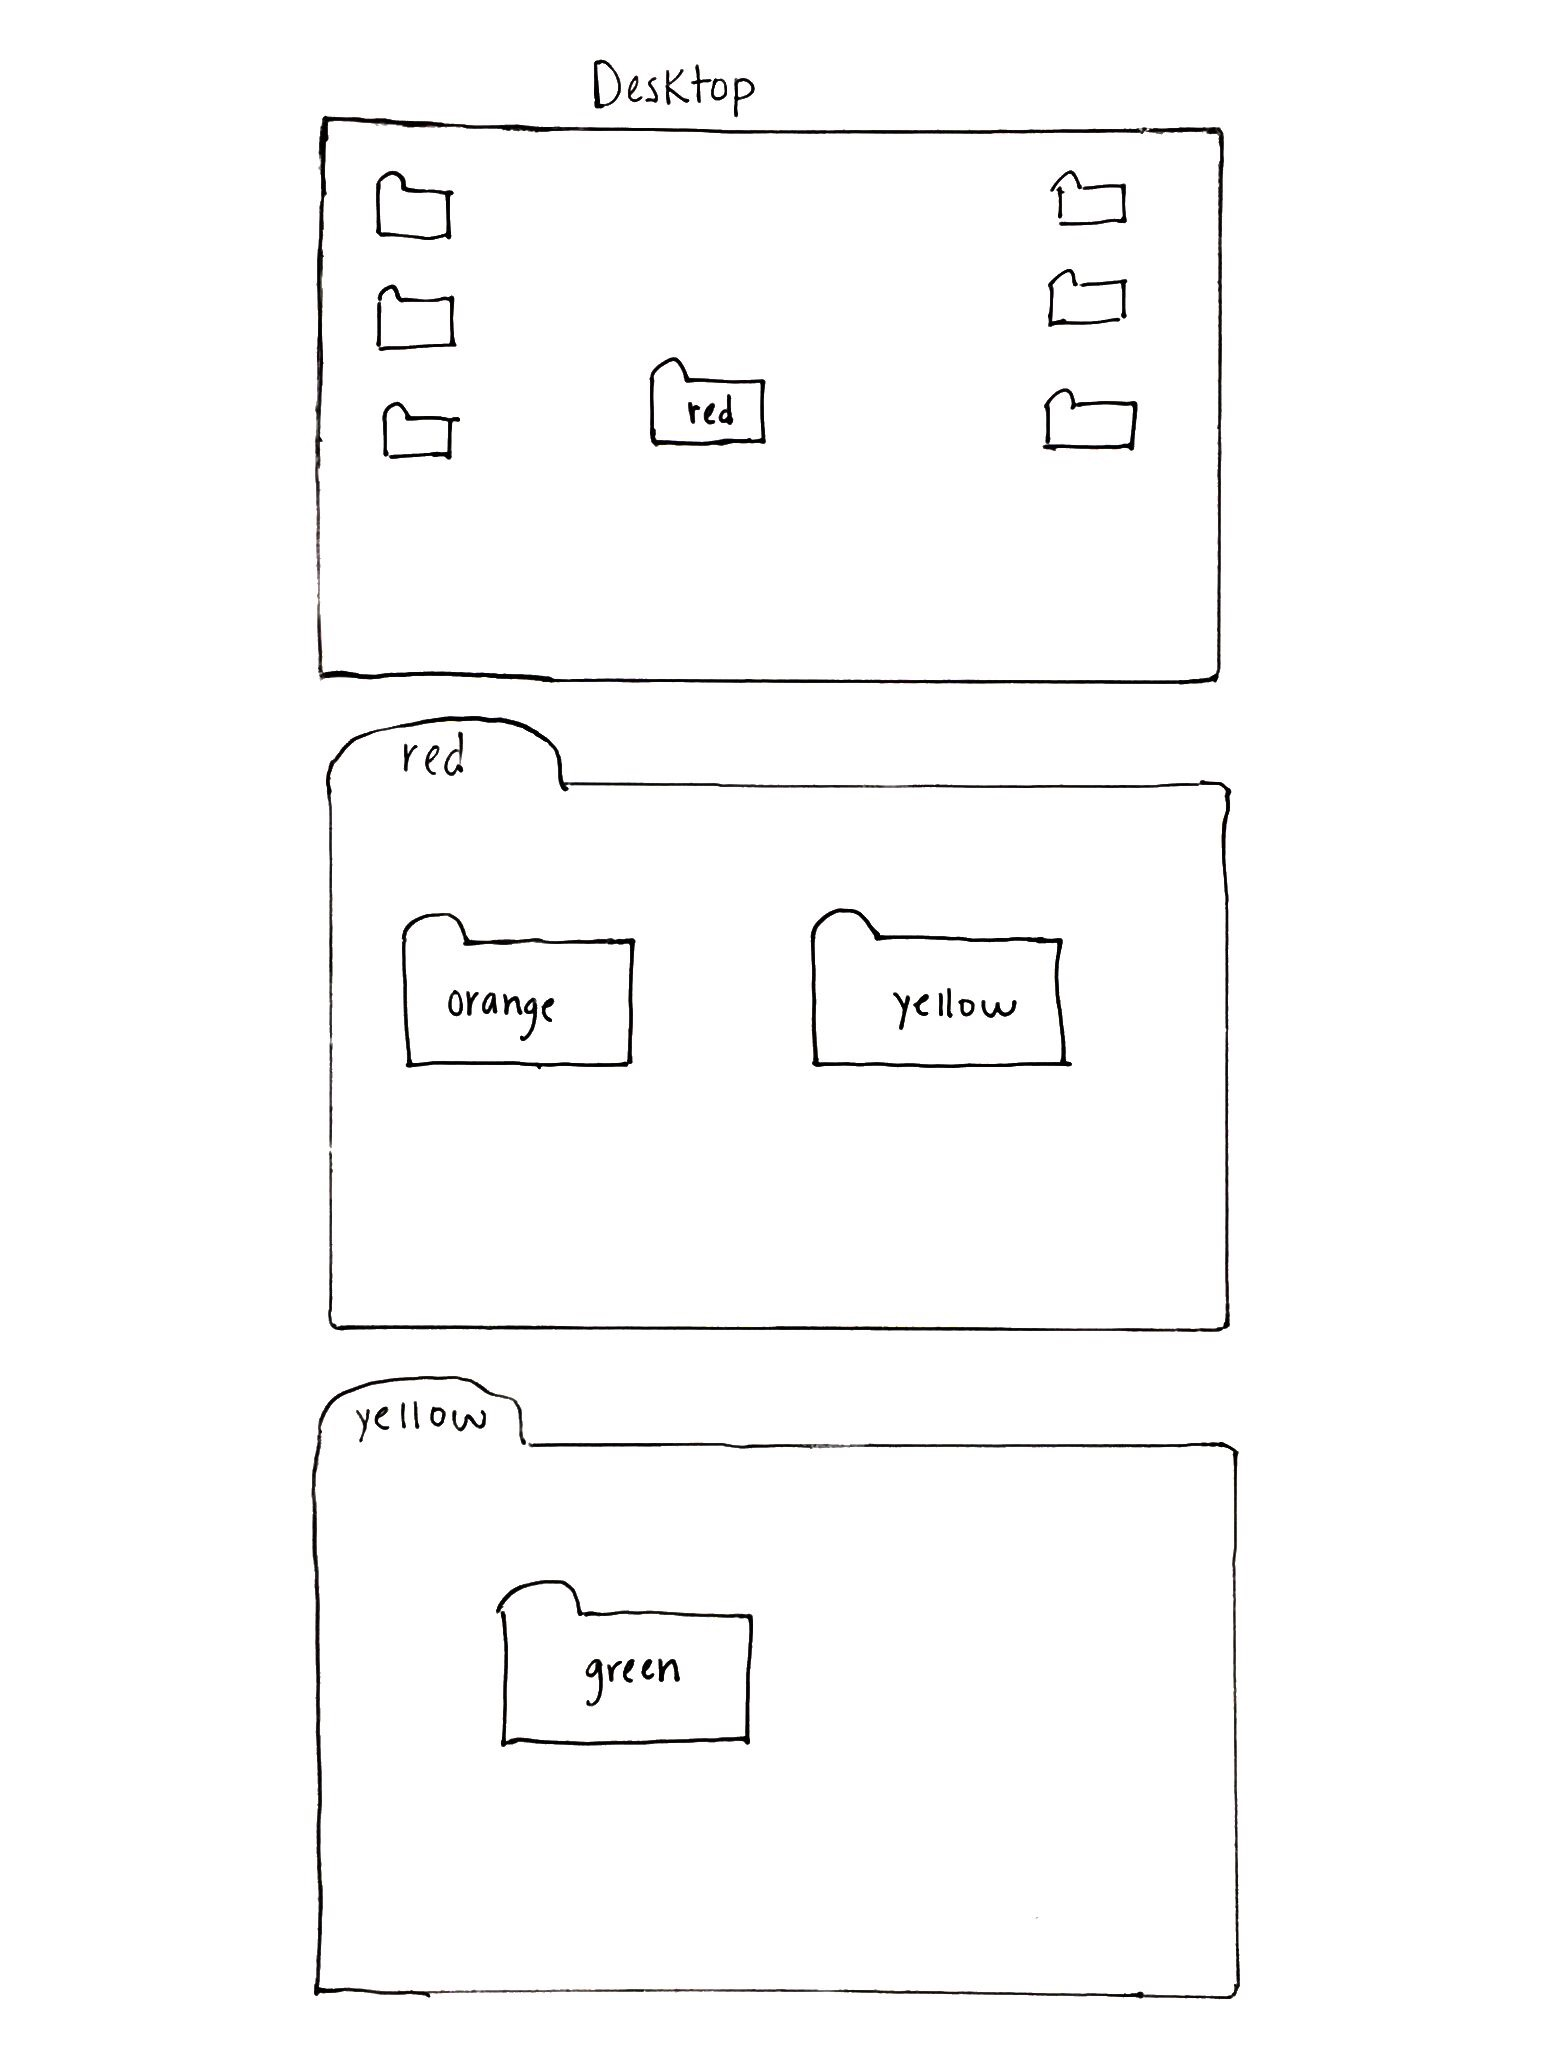
\includegraphics{~/Desktop/fp1.jpg} 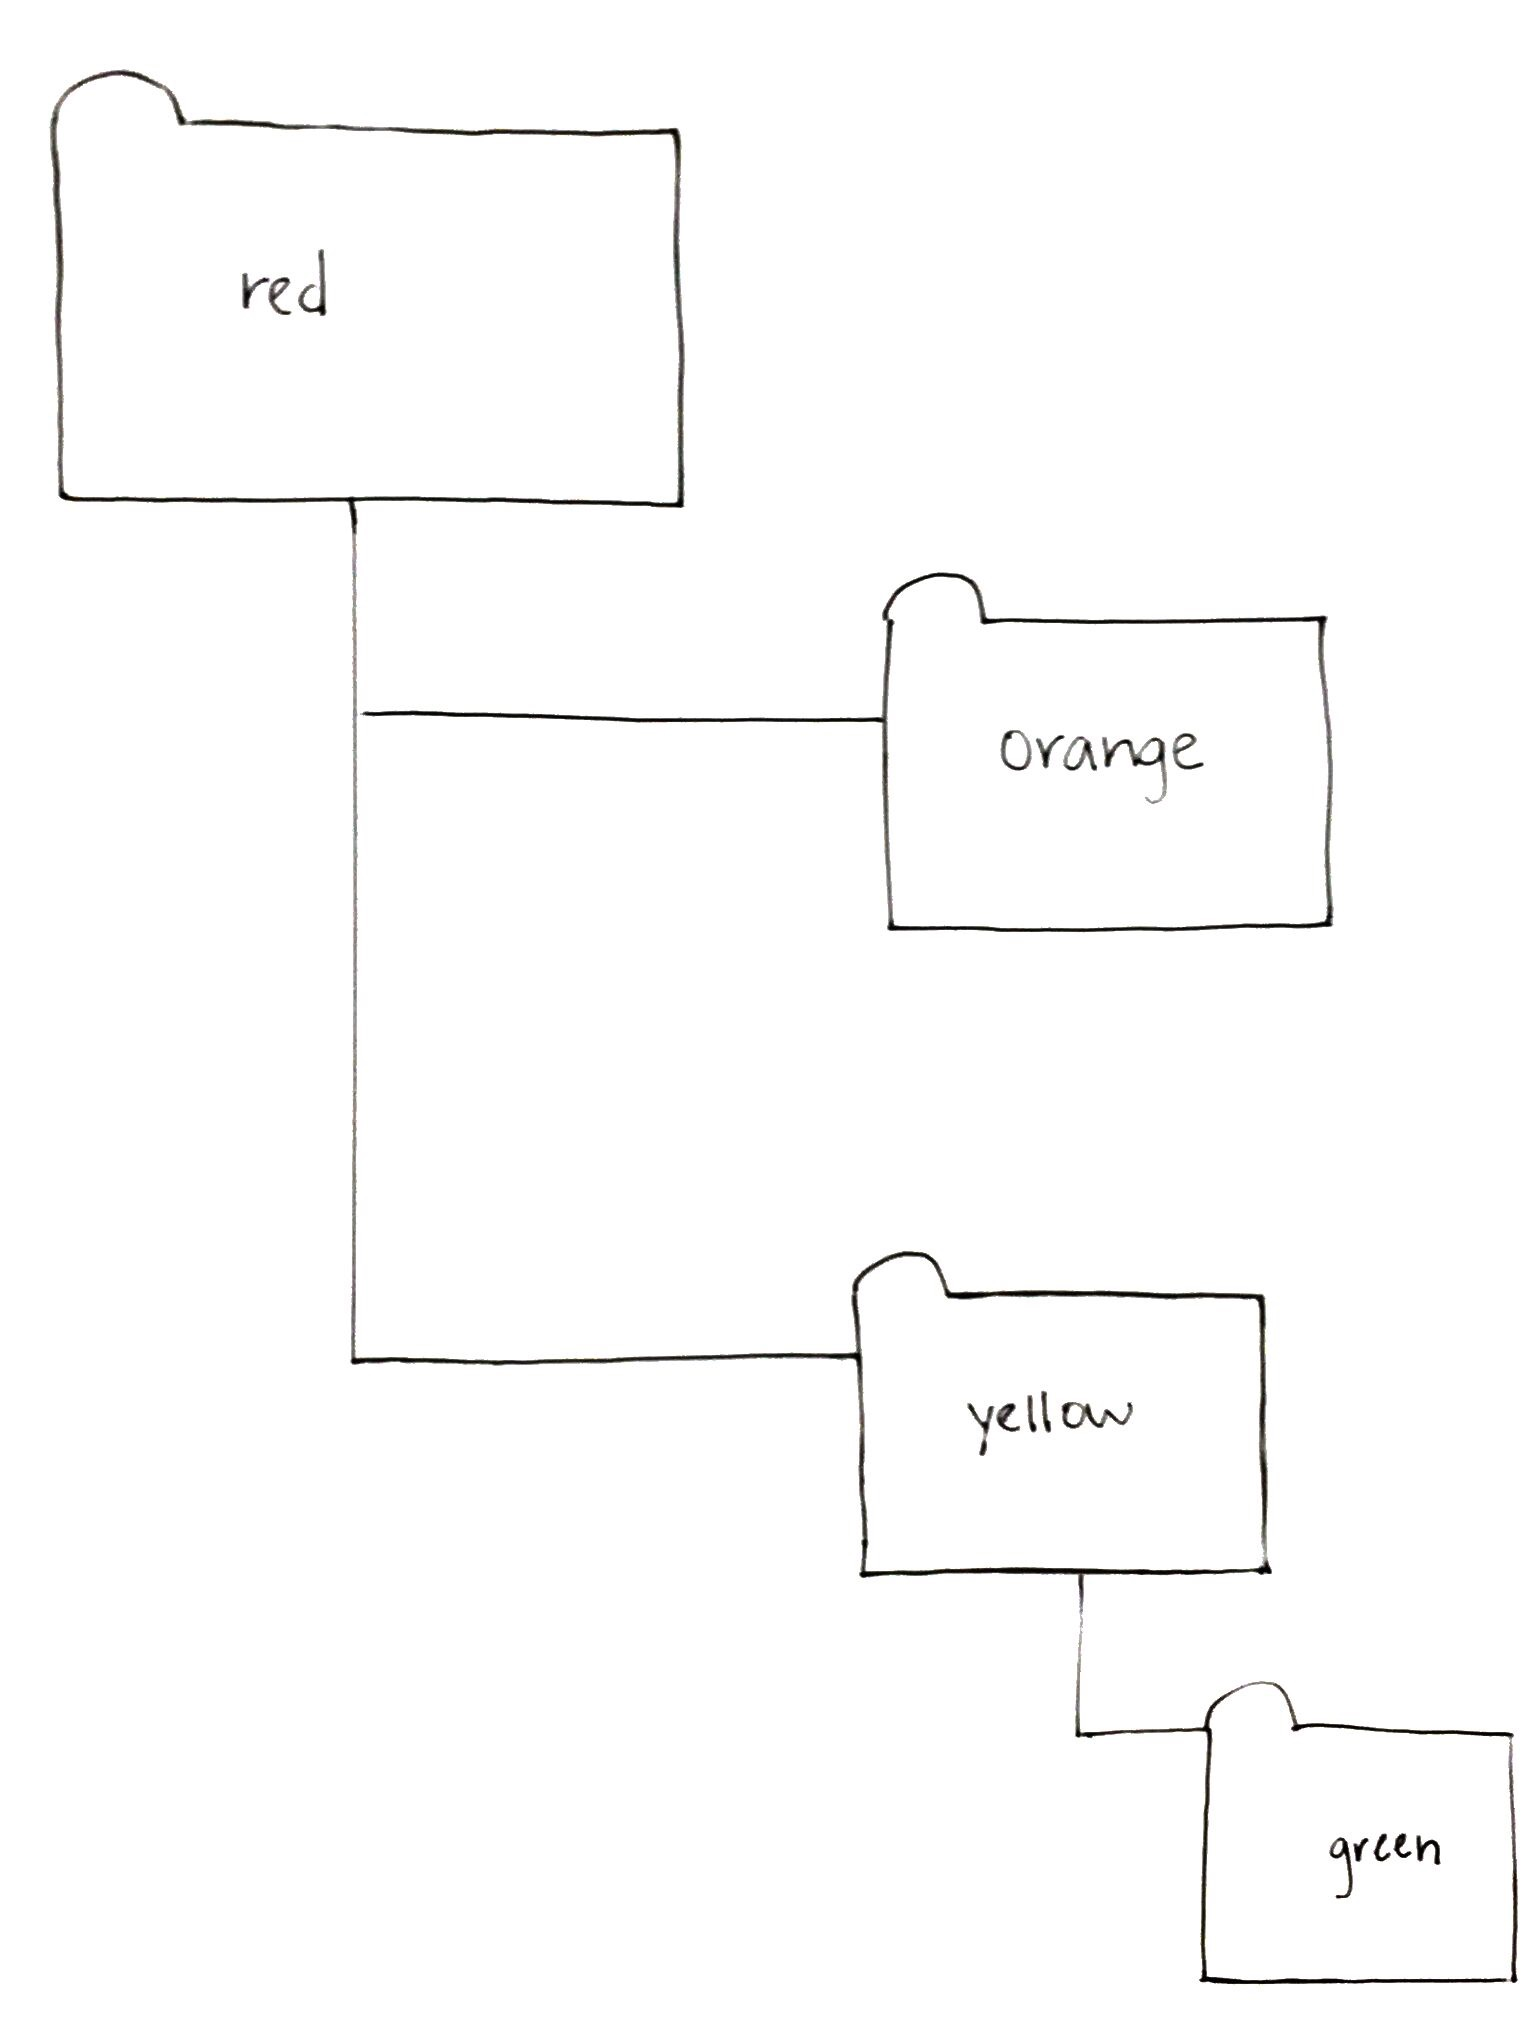
\includegraphics{~/Desktop/fp2.jpg}

\end{frame}

\begin{frame}[fragile]{Exercise continued}

Let's say we want to get to the green folder using the absolute file
path.\\
1. View your current working directory \texttt{getwd()}\\
2. Set your working directory to the green folder using the absolute
file path\\
3. Now set your working directory to the orange folder using the
relative file path (hint: ../)

\end{frame}

\begin{frame}[fragile]{Solution}

\begin{Shaded}
\begin{Highlighting}[]
\KeywordTok{getwd}\NormalTok{()}
\CommentTok{#> [1] "/Users/patriciamartin/Desktop/GitHub/rclass/lectures/lecture2"}
\KeywordTok{setwd}\NormalTok{(}\StringTok{"~/Desktop/red/yellow/green"}\NormalTok{)}
\KeywordTok{getwd}\NormalTok{() }
\CommentTok{#> [1] "/Users/patriciamartin/Desktop/red/yellow/green"}
\KeywordTok{setwd}\NormalTok{(}\StringTok{"../../orange"}\NormalTok{)}
\KeywordTok{getwd}\NormalTok{()}
\CommentTok{#> [1] "/Users/patriciamartin/Desktop/red/orange"}
\end{Highlighting}
\end{Shaded}

\end{frame}

\section{Investigating objects, Base R
approach}\label{investigating-objects-base-r-approach}

\begin{frame}[fragile]{Load .Rdata data frames we will use today}

Data on off-campus recruiting events by public universities

\begin{itemize}
\tightlist
\item
  Data frame object \texttt{df\_event}

  \begin{itemize}
  \tightlist
  \item
    One observation per university, recruiting event
  \end{itemize}
\item
  Data frame object \texttt{df\_school}

  \begin{itemize}
  \tightlist
  \item
    One observation per high school (visited and non-visited)
  \end{itemize}
\end{itemize}

\begin{Shaded}
\begin{Highlighting}[]
\KeywordTok{rm}\NormalTok{(}\DataTypeTok{list =} \KeywordTok{ls}\NormalTok{()) }\CommentTok{# remove all objects in current environment}

\KeywordTok{getwd}\NormalTok{()}
\CommentTok{#> [1] "/Users/patriciamartin/Desktop/GitHub/rclass/lectures/lecture2"}
\CommentTok{#load dataset with one obs per recruiting event}
\KeywordTok{load}\NormalTok{(}\KeywordTok{url}\NormalTok{(}\StringTok{"https://github.com/ozanj/rclass/raw/master/data/recruiting/recruit_event_somevars.RData"}\NormalTok{))}
\CommentTok{#load("../../data/recruiting/recruit_event_somevars.Rdata")}

\CommentTok{#load dataset with one obs per high school}
\KeywordTok{load}\NormalTok{(}\KeywordTok{url}\NormalTok{(}\StringTok{"https://github.com/ozanj/rclass/raw/master/data/recruiting/recruit_school_somevars.RData"}\NormalTok{))}
\CommentTok{#load("../../data/recruiting/recruit_school_somevars.Rdata")}
\end{Highlighting}
\end{Shaded}

\end{frame}

\begin{frame}[fragile]{Listing objects}

\textbf{Files in your working directory}

\texttt{list.files()} function lists files in your current working
directory

\begin{itemize}
\tightlist
\item
  if you run this code from .Rmd file, working directory is location
  .Rmd file is stored
\end{itemize}

\begin{Shaded}
\begin{Highlighting}[]
\KeywordTok{getwd}\NormalTok{() }\CommentTok{# what is your current working directory}
\CommentTok{#> [1] "/Users/patriciamartin/Desktop/GitHub/rclass/lectures/lecture2"}
\KeywordTok{list.files}\NormalTok{()}
\CommentTok{#> [1] "fp1.JPG"                     "fp2.JPG"                    }
\CommentTok{#> [3] "lecture2.pdf"                "lecture2.Rmd"               }
\CommentTok{#> [5] "lecture2.tex"                "sample_simple_rmarkdown.txt"}
\CommentTok{#> [7] "sample.Rmd"                  "text"                       }
\CommentTok{#> [9] "transform-logical.png"}
\end{Highlighting}
\end{Shaded}

\textbf{Objects currently open in your R session}

\texttt{ls()} function lists objects currently open in R

\begin{Shaded}
\begin{Highlighting}[]
\NormalTok{x <-}\StringTok{ "hello!"}
\KeywordTok{ls}\NormalTok{() }\CommentTok{# Objects open in R}
\CommentTok{#> [1] "df_event"  "df_school" "x"}
\end{Highlighting}
\end{Shaded}

\end{frame}

\begin{frame}[fragile]{Removing objects}

\texttt{rm()} function removes specified objects open in R

\begin{Shaded}
\begin{Highlighting}[]
\KeywordTok{rm}\NormalTok{(x)}
\KeywordTok{ls}\NormalTok{()}
\CommentTok{#> [1] "df_event"  "df_school"}
\end{Highlighting}
\end{Shaded}

Command to remove all objects open in R (I don't run it)

\begin{Shaded}
\begin{Highlighting}[]
\KeywordTok{rm}\NormalTok{(}\DataTypeTok{list =} \KeywordTok{ls}\NormalTok{())}
\end{Highlighting}
\end{Shaded}

\end{frame}

\begin{frame}[fragile]{Describing objects, focus on \textbf{data
frames}}

\medskip \textbf{type} and \textbf{length} of a data frame object

\begin{itemize}
\tightlist
\item
  Recall that a data frame is an object where \textbf{type} is a list
\item
  \textbf{Length} of an object is the number of elements

  \begin{itemize}
  \tightlist
  \item
    When object is a data frame, number of elements = number of
    variables
  \end{itemize}
\end{itemize}

\begin{Shaded}
\begin{Highlighting}[]
\KeywordTok{typeof}\NormalTok{(df_event)}
\CommentTok{#> [1] "list"}
\KeywordTok{length}\NormalTok{(df_event) }\CommentTok{# = num elements = num columns}
\CommentTok{#> [1] 33}
\end{Highlighting}
\end{Shaded}

Number of \textbf{columns} and \textbf{rows} of data frame object

\begin{itemize}
\tightlist
\item
  number of columns = number of elements = number of variables
\item
  number of rows = number of observations
\end{itemize}

\begin{Shaded}
\begin{Highlighting}[]
\KeywordTok{ncol}\NormalTok{(df_event) }\CommentTok{# num columns = num variables}
\CommentTok{#> [1] 33}
\KeywordTok{nrow}\NormalTok{(df_event) }\CommentTok{# num rows = num observations}
\CommentTok{#> [1] 17976}
\KeywordTok{dim}\NormalTok{(df_event) }\CommentTok{# shows number rows by columns}
\CommentTok{#> [1] 17976    33}
\end{Highlighting}
\end{Shaded}

\texttt{str()} provides compact information on structure any object
(output omitted)

\begin{Shaded}
\begin{Highlighting}[]
\KeywordTok{str}\NormalTok{(df_event)}
\end{Highlighting}
\end{Shaded}

\end{frame}

\subsection{Variables names}\label{variables-names}

\begin{frame}[fragile]{Variable names}

\texttt{names()} function lists names of elements in an object

\begin{Shaded}
\begin{Highlighting}[]
\NormalTok{?names}
\end{Highlighting}
\end{Shaded}

When object is a data frame:

\begin{itemize}
\tightlist
\item
  each element is a variable
\item
  each element name is a variable name
\end{itemize}

\begin{Shaded}
\begin{Highlighting}[]
\KeywordTok{names}\NormalTok{(df_event)}
\CommentTok{#>  [1] "instnm"               "univ_id"              "instst"              }
\CommentTok{#>  [4] "pid"                  "event_date"           "event_type"          }
\CommentTok{#>  [7] "zip"                  "school_id"            "ipeds_id"            }
\CommentTok{#> [10] "event_state"          "event_inst"           "med_inc"             }
\CommentTok{#> [13] "pop_total"            "pct_white_zip"        "pct_black_zip"       }
\CommentTok{#> [16] "pct_asian_zip"        "pct_hispanic_zip"     "pct_amerindian_zip"  }
\CommentTok{#> [19] "pct_nativehawaii_zip" "pct_tworaces_zip"     "pct_otherrace_zip"   }
\CommentTok{#> [22] "fr_lunch"             "titlei_status_pub"    "total_12"            }
\CommentTok{#> [25] "school_type_pri"      "school_type_pub"      "g12offered"          }
\CommentTok{#> [28] "g12"                  "total_students_pub"   "total_students_pri"  }
\CommentTok{#> [31] "event_name"           "event_location_name"  "event_datetime_start"}
\end{Highlighting}
\end{Shaded}

\end{frame}

\begin{frame}[fragile]{Variable names}

Refer to specific named elements of an object using this syntax:

\begin{itemize}
\tightlist
\item
  \texttt{obj\_name\$element\_name}
\end{itemize}

When object is data frame, refer to specific variables using this
syntax:

\begin{itemize}
\tightlist
\item
  \texttt{data\_fram\_name\$varname}
\item
  \textbf{This approach to isolating variables very useful for
  investigating data}
\end{itemize}

\begin{Shaded}
\begin{Highlighting}[]
\KeywordTok{typeof}\NormalTok{(df_event}\OperatorTok{$}\NormalTok{instnm)}
\CommentTok{#> [1] "character"}
\KeywordTok{typeof}\NormalTok{(df_event}\OperatorTok{$}\NormalTok{med_inc)}
\CommentTok{#> [1] "double"}
\end{Highlighting}
\end{Shaded}

\end{frame}

\begin{frame}[fragile]{Variable names}

\medskip Recall that data frames are lists with following criteria:

\begin{itemize}
\tightlist
\item
  each element of the list is a vector

  \begin{itemize}
  \tightlist
  \item
    each element of list is a variable; length of data frame = number of
    variables
  \end{itemize}
\end{itemize}

\begin{Shaded}
\begin{Highlighting}[]
\KeywordTok{length}\NormalTok{(df_event)}
\CommentTok{#> [1] 33}
\KeywordTok{nrow}\NormalTok{(df_event)}
\CommentTok{#> [1] 17976}
\CommentTok{#str(df_event)}
\end{Highlighting}
\end{Shaded}

\begin{itemize}
\tightlist
\item
  each element of the list (i.e., variable) has the same length

  \begin{itemize}
  \tightlist
  \item
    Length of each variable is equal to number of observations in data
    frame
  \end{itemize}
\end{itemize}

\begin{Shaded}
\begin{Highlighting}[]
\KeywordTok{typeof}\NormalTok{(df_event}\OperatorTok{$}\NormalTok{event_state)}
\CommentTok{#> [1] "character"}
\KeywordTok{length}\NormalTok{(df_event}\OperatorTok{$}\NormalTok{event_state)}
\CommentTok{#> [1] 17976}
\KeywordTok{str}\NormalTok{(df_event}\OperatorTok{$}\NormalTok{event_state)}
\CommentTok{#>  chr [1:17976] "MA" "MA" "MA" "MA" "MA" "MA" "MA" "MA" "MA" "MA" "MA" ...}

\KeywordTok{typeof}\NormalTok{(df_event}\OperatorTok{$}\NormalTok{med_inc)}
\CommentTok{#> [1] "double"}
\KeywordTok{length}\NormalTok{(df_event}\OperatorTok{$}\NormalTok{med_inc)}
\CommentTok{#> [1] 17976}
\KeywordTok{str}\NormalTok{(df_event}\OperatorTok{$}\NormalTok{med_inc)}
\CommentTok{#>  num [1:17976] 71714 89122 70136 70136 71024 ...}
\end{Highlighting}
\end{Shaded}

\end{frame}

\subsection{View and print data}\label{view-and-print-data}

\begin{frame}[fragile]{Viewing and printing data frames}

Three ways to view/print a data frame object

\begin{enumerate}
\def\labelenumi{\arabic{enumi}.}
\item
  Simply type the object name (output omitted)

  \begin{itemize}
  \tightlist
  \item
    number of observations and rows printed depend on YAML header
    settings and on attributes (discussed next week) of the object
  \end{itemize}
\end{enumerate}

\begin{Shaded}
\begin{Highlighting}[]
\NormalTok{df_event}
\end{Highlighting}
\end{Shaded}

\begin{enumerate}
\def\labelenumi{\arabic{enumi}.}
\setcounter{enumi}{1}
\tightlist
\item
  Use the \texttt{View()} function to view data in a browser
\end{enumerate}

\begin{Shaded}
\begin{Highlighting}[]
\KeywordTok{View}\NormalTok{(df_event)}
\end{Highlighting}
\end{Shaded}

\begin{enumerate}
\def\labelenumi{\arabic{enumi}.}
\setcounter{enumi}{2}
\tightlist
\item
  \texttt{head()} to show the first \emph{n} rows
\end{enumerate}

\begin{Shaded}
\begin{Highlighting}[]
\CommentTok{#?head}
\KeywordTok{head}\NormalTok{(df_event, }\DataTypeTok{n=}\DecValTok{5}\NormalTok{)}
\end{Highlighting}
\end{Shaded}

\end{frame}

\begin{frame}[fragile]{Viewing and printing data frames}

\texttt{obj\_name{[}\textless{}rows\textgreater{},\textless{}cols\textgreater{}{]}}
to print specific rows and columns of data frame

\begin{itemize}
\tightlist
\item
  particularly powerful when combined with sequences (e.g.,
  \texttt{1:10})
\end{itemize}

\medskip Examples:

\begin{itemize}
\tightlist
\item
  Print first five rows
\end{itemize}

\begin{Shaded}
\begin{Highlighting}[]
\NormalTok{df_event[}\DecValTok{1}\OperatorTok{:}\DecValTok{5}\NormalTok{, ]}
\end{Highlighting}
\end{Shaded}

\begin{itemize}
\tightlist
\item
  Print first five rows and first three columns
\end{itemize}

\begin{Shaded}
\begin{Highlighting}[]
\NormalTok{df_event[}\DecValTok{1}\OperatorTok{:}\DecValTok{5}\NormalTok{, }\DecValTok{1}\OperatorTok{:}\DecValTok{3}\NormalTok{]}
\end{Highlighting}
\end{Shaded}

\begin{itemize}
\tightlist
\item
  Print first three columns of the 100th observation
\end{itemize}

\begin{Shaded}
\begin{Highlighting}[]
\NormalTok{df_event[}\DecValTok{100}\NormalTok{, }\DecValTok{1}\OperatorTok{:}\DecValTok{3}\NormalTok{]}
\end{Highlighting}
\end{Shaded}

\begin{itemize}
\tightlist
\item
  Print the 50th observation, all variables
\end{itemize}

\begin{Shaded}
\begin{Highlighting}[]
\NormalTok{df_event[}\DecValTok{50}\NormalTok{,]}
\end{Highlighting}
\end{Shaded}

\end{frame}

\begin{frame}[fragile]{Viewing and printing data}

type \texttt{obj\_name\$var\_name} to print specific elements (i.e.,
variables) in a data frame

\begin{Shaded}
\begin{Highlighting}[]
\NormalTok{df_event}\OperatorTok{$}\NormalTok{zip}
\end{Highlighting}
\end{Shaded}

\begin{itemize}
\tightlist
\item
  recall that these elements are vectors, with length = number of obs
\end{itemize}

\begin{Shaded}
\begin{Highlighting}[]
\KeywordTok{typeof}\NormalTok{(df_event}\OperatorTok{$}\NormalTok{zip)}
\CommentTok{#> [1] "character"}
\KeywordTok{length}\NormalTok{(df_event}\OperatorTok{$}\NormalTok{zip)}
\CommentTok{#> [1] 17976}
\end{Highlighting}
\end{Shaded}

\begin{itemize}
\tightlist
\item
  \texttt{obj\_name\$var\_name} syntax can be combined with sequences

  \begin{itemize}
  \tightlist
  \item
    vectors don't have ``rows'' or ``columns''; they just have elements
  \item
    so use sequence to identify which elements you want to print
  \end{itemize}
\end{itemize}

\begin{Shaded}
\begin{Highlighting}[]
\NormalTok{df_event}\OperatorTok{$}\NormalTok{event_state[}\DecValTok{1}\OperatorTok{:}\DecValTok{10}\NormalTok{]}
\CommentTok{#>  [1] "MA" "MA" "MA" "MA" "MA" "MA" "MA" "MA" "MA" "MA"}
\NormalTok{df_event}\OperatorTok{$}\NormalTok{event_type[}\DecValTok{6}\OperatorTok{:}\DecValTok{10}\NormalTok{]}
\CommentTok{#> [1] "private hs" "public hs"  "private hs" "public hs"  "public hs"}
\end{Highlighting}
\end{Shaded}

\begin{itemize}
\tightlist
\item
  can also print multiple variables using \texttt{combine()} function
\end{itemize}

\begin{Shaded}
\begin{Highlighting}[]
\KeywordTok{c}\NormalTok{(df_event}\OperatorTok{$}\NormalTok{event_state[}\DecValTok{1}\OperatorTok{:}\DecValTok{5}\NormalTok{],df_event}\OperatorTok{$}\NormalTok{event_type[}\DecValTok{1}\OperatorTok{:}\DecValTok{5}\NormalTok{])}
\CommentTok{#>  [1] "MA"         "MA"         "MA"         "MA"         "MA"        }
\CommentTok{#>  [6] "public hs"  "public hs"  "public hs"  "public hs"  "private hs"}
\end{Highlighting}
\end{Shaded}

\end{frame}

\begin{frame}[fragile]{Exercise}

Create a printing exercise using the df\_school

\begin{enumerate}
\def\labelenumi{\arabic{enumi}.}
\tightlist
\item
  Use
  \texttt{obj\_name{[}\textless{}rows\textgreater{},\textless{}cols\textgreater{}{]}}
  to print the first 5 rows and 3 columns of data frame
\item
  Use head() to print first 4 observations
\item
  Use \texttt{obj\_name\$var\_name{[}1:10{]}} to print the first 10
  observations of a variable
\item
  Use combine() to print the first 3 observations of variables
  ``school\_type'' \& ``name''
\end{enumerate}

\end{frame}

\begin{frame}[fragile]{Solution}

\begin{enumerate}
\def\labelenumi{\arabic{enumi}.}
\tightlist
\item
  Use
  \texttt{obj\_name{[}\textless{}rows\textgreater{},\textless{}cols\textgreater{}{]}}
  to print the first 5 rows and 3 columns of data frame
\end{enumerate}

\begin{Shaded}
\begin{Highlighting}[]
\NormalTok{df_school[}\DecValTok{1}\OperatorTok{:}\DecValTok{5}\NormalTok{,}\DecValTok{1}\OperatorTok{:}\DecValTok{3}\NormalTok{]}
\CommentTok{#> # A tibble: 5 x 3}
\CommentTok{#>   state_code school_type ncessch     }
\CommentTok{#>   <chr>      <chr>       <chr>       }
\CommentTok{#> 1 AK         public      020000100208}
\CommentTok{#> 2 AK         public      020000100211}
\CommentTok{#> 3 AK         public      020000100212}
\CommentTok{#> 4 AK         public      020000100213}
\CommentTok{#> 5 AK         public      020000300216}
\end{Highlighting}
\end{Shaded}

\end{frame}

\begin{frame}[fragile]{Solution}

\begin{enumerate}
\def\labelenumi{\arabic{enumi}.}
\setcounter{enumi}{1}
\tightlist
\item
  Use head() to print first 4 observations
\end{enumerate}

\begin{Shaded}
\begin{Highlighting}[]
\KeywordTok{head}\NormalTok{(df_school, }\DataTypeTok{n=}\DecValTok{4}\NormalTok{)}
\CommentTok{#> # A tibble: 4 x 26}
\CommentTok{#>   state_code school_type ncessch name  address city  zip_code pct_white}
\CommentTok{#>   <chr>      <chr>       <chr>   <chr> <chr>   <chr> <chr>        <dbl>}
\CommentTok{#> 1 AK         public      020000~ Beth~ 1006 R~ Beth~ 99559         11.8}
\CommentTok{#> 2 AK         public      020000~ Ayag~ 106 Vi~ Kong~ 99559          0  }
\CommentTok{#> 3 AK         public      020000~ Kwig~ 108 Vi~ Kwig~ 99622          0  }
\CommentTok{#> 4 AK         public      020000~ Nels~ 118 Vi~ Toks~ 99637          0  }
\CommentTok{#> # ... with 18 more variables: pct_black <dbl>, pct_hispanic <dbl>,}
\CommentTok{#> #   pct_asian <dbl>, pct_amerindian <dbl>, pct_other <dbl>,}
\CommentTok{#> #   num_fr_lunch <dbl>, total_students <dbl>, num_took_math <dbl>,}
\CommentTok{#> #   num_prof_math <dbl>, num_took_rla <dbl>, num_prof_rla <dbl>,}
\CommentTok{#> #   avgmedian_inc_2564 <dbl>, visits_by_110635 <int>,}
\CommentTok{#> #   visits_by_126614 <int>, visits_by_100751 <int>, inst_110635 <chr>,}
\CommentTok{#> #   inst_126614 <chr>, inst_100751 <chr>}
\end{Highlighting}
\end{Shaded}

\end{frame}

\begin{frame}[fragile]{Solution}

\begin{enumerate}
\def\labelenumi{\arabic{enumi}.}
\setcounter{enumi}{2}
\tightlist
\item
  Use \texttt{obj\_name\$var\_name{[}1:10{]}} to print the first 10
  observations of a variable
\end{enumerate}

\begin{Shaded}
\begin{Highlighting}[]
\NormalTok{df_school}\OperatorTok{$}\NormalTok{name[}\DecValTok{1}\OperatorTok{:}\DecValTok{10}\NormalTok{]}
\CommentTok{#>  [1] "Bethel Regional High School" "Ayagina'ar Elitnaurvik"     }
\CommentTok{#>  [3] "Kwigillingok School"         "Nelson Island Area School"  }
\CommentTok{#>  [5] "Alakanuk School"             "Emmonak School"             }
\CommentTok{#>  [7] "Hooper Bay School"           "Ignatius Beans School"      }
\CommentTok{#>  [9] "Pilot Station School"        "Kotlik School"}
\end{Highlighting}
\end{Shaded}

\end{frame}

\begin{frame}[fragile]{Solution}

\begin{enumerate}
\def\labelenumi{\arabic{enumi}.}
\setcounter{enumi}{3}
\tightlist
\item
  Use combine() to print the first 3 observations of variables
  ``school\_type'' \& ``name''
\end{enumerate}

\begin{Shaded}
\begin{Highlighting}[]
\KeywordTok{c}\NormalTok{(df_school}\OperatorTok{$}\NormalTok{school_type[}\DecValTok{1}\OperatorTok{:}\DecValTok{3}\NormalTok{],df_school}\OperatorTok{$}\NormalTok{name[}\DecValTok{1}\OperatorTok{:}\DecValTok{3}\NormalTok{])}
\CommentTok{#> [1] "public"                      "public"                     }
\CommentTok{#> [3] "public"                      "Bethel Regional High School"}
\CommentTok{#> [5] "Ayagina'ar Elitnaurvik"      "Kwigillingok School"}
\end{Highlighting}
\end{Shaded}

\end{frame}

\subsection{Missing values}\label{missing-values}

\begin{frame}[fragile]{Missing values}

Missing values have the value \texttt{NA}

\begin{itemize}
\tightlist
\item
  \texttt{NA} is a special keyword, not the same as the character string
  \texttt{"NA"}
\end{itemize}

use \texttt{is.na()} function to determine if a value is missing

\begin{itemize}
\tightlist
\item
  \texttt{is.na()} returns a logical vector
\end{itemize}

\begin{Shaded}
\begin{Highlighting}[]
\KeywordTok{is.na}\NormalTok{(}\DecValTok{5}\NormalTok{)}
\CommentTok{#> [1] FALSE}
\KeywordTok{is.na}\NormalTok{(}\OtherTok{NA}\NormalTok{)}
\CommentTok{#> [1] TRUE}
\KeywordTok{is.na}\NormalTok{(}\StringTok{"NA"}\NormalTok{)}
\CommentTok{#> [1] FALSE}
\KeywordTok{typeof}\NormalTok{(}\KeywordTok{is.na}\NormalTok{(}\StringTok{"NA"}\NormalTok{)) }\CommentTok{# example of a logical vector}
\CommentTok{#> [1] "logical"}

\NormalTok{nvector <-}\StringTok{ }\KeywordTok{c}\NormalTok{(}\DecValTok{10}\NormalTok{,}\DecValTok{5}\NormalTok{,}\OtherTok{NA}\NormalTok{)}
\KeywordTok{is.na}\NormalTok{(nvector)}
\CommentTok{#> [1] FALSE FALSE  TRUE}
\KeywordTok{typeof}\NormalTok{(}\KeywordTok{is.na}\NormalTok{(nvector)) }\CommentTok{# example of a logical vector}
\CommentTok{#> [1] "logical"}

\NormalTok{svector <-}\StringTok{ }\KeywordTok{c}\NormalTok{(}\StringTok{"e"}\NormalTok{,}\StringTok{"f"}\NormalTok{,}\OtherTok{NA}\NormalTok{,}\StringTok{"NA"}\NormalTok{)}
\KeywordTok{is.na}\NormalTok{(svector)}
\CommentTok{#> [1] FALSE FALSE  TRUE FALSE}
\end{Highlighting}
\end{Shaded}

\end{frame}

\begin{frame}[fragile]{Missing values are ``contageous''}

What does ``contageous'' mean?

\begin{itemize}
\tightlist
\item
  operations involving a missing value will yield a missing value
\end{itemize}

\begin{Shaded}
\begin{Highlighting}[]
\DecValTok{7}\OperatorTok{>}\DecValTok{5}
\CommentTok{#> [1] TRUE}
\DecValTok{7}\OperatorTok{>}\OtherTok{NA}
\CommentTok{#> [1] NA}
\DecValTok{0}\OperatorTok{==}\OtherTok{NA}
\CommentTok{#> [1] NA}
\DecValTok{2}\OperatorTok{*}\KeywordTok{c}\NormalTok{(}\DecValTok{0}\NormalTok{,}\DecValTok{1}\NormalTok{,}\DecValTok{2}\NormalTok{,}\OtherTok{NA}\NormalTok{)}
\CommentTok{#> [1]  0  2  4 NA}
\OtherTok{NA}\OperatorTok{*}\KeywordTok{c}\NormalTok{(}\DecValTok{0}\NormalTok{,}\DecValTok{1}\NormalTok{,}\DecValTok{2}\NormalTok{,}\OtherTok{NA}\NormalTok{)}
\CommentTok{#> [1] NA NA NA NA}
\end{Highlighting}
\end{Shaded}

\end{frame}

\begin{frame}[fragile]{Function and missing values, the \texttt{table()}
function}

\texttt{table()} function useful for investigating categorical variables

\begin{Shaded}
\begin{Highlighting}[]
\KeywordTok{table}\NormalTok{(df_event}\OperatorTok{$}\NormalTok{g12offered)}
\CommentTok{#> }
\CommentTok{#>     1 }
\CommentTok{#> 11025}
\end{Highlighting}
\end{Shaded}

By default \texttt{table()} ignores \texttt{NA} values

\begin{itemize}
\tightlist
\item
  \texttt{useNA} argument determines whether to include \texttt{NA}
  values

  \begin{itemize}
  \tightlist
  \item
    ``allowed values correspond to never (''no``); only if count is
    positive (''ifany``); and even for zero counts (''always``)''
  \end{itemize}
\end{itemize}

\begin{Shaded}
\begin{Highlighting}[]
\KeywordTok{nrow}\NormalTok{(df_event)}
\CommentTok{#> [1] 17976}
\KeywordTok{table}\NormalTok{(df_event}\OperatorTok{$}\NormalTok{g12offered, }\DataTypeTok{useNA=}\StringTok{"always"}\NormalTok{)}
\CommentTok{#> }
\CommentTok{#>     1  <NA> }
\CommentTok{#> 11025  6951}
\end{Highlighting}
\end{Shaded}

Broader point:

\begin{itemize}
\tightlist
\item
  Most functions that create descriptive statistics have options about
  how to treat missing values
\item
  When investigating data, good practice to \emph{always} show missing
  values
\end{itemize}

Tip:

\begin{itemize}
\tightlist
\item
  command \texttt{str(df\_event)} shows which variables have missing
  values
\end{itemize}

\end{frame}

\section{Investigating data frames, tidyverse
approach}\label{investigating-data-frames-tidyverse-approach}

\begin{frame}[fragile]{Introduction to the \texttt{dplyr} library}

\texttt{dplyr}, a package within the \texttt{tidyverse} suite of
packages, provide tools for manipulating data frames

\begin{itemize}
\tightlist
\item
  Wickham describes functions within \texttt{dplyr} as a set of
  ``verbs'' that fall in the broader categories of \textbf{subsetting},
  \textbf{sorting}, and \textbf{transforming}
\end{itemize}

\begin{longtable}[]{@{}ll@{}}
\toprule
Today & Next two weeks\tabularnewline
\midrule
\endhead
\textbf{Subsetting data} & \textbf{Transforming data}\tabularnewline
- \texttt{select()} variables & - \texttt{mutate()} creates new
variables\tabularnewline
- \texttt{filter()} observations & - \texttt{summarize()} calculates
across rows\tabularnewline
\textbf{Sorting data} & - \texttt{group\_by()} to calculate across rows
within groups\tabularnewline
- \texttt{arrange()} &\tabularnewline
\bottomrule
\end{longtable}

All \texttt{dplyr} verbs (i.e., functions) work as follows

\begin{enumerate}
\def\labelenumi{\arabic{enumi}.}
\tightlist
\item
  first argument is a data frame
\item
  subsequent arguments describe what to do with variables and
  observations in data frame

  \begin{itemize}
  \tightlist
  \item
    refer to variable names without quotes
  \end{itemize}
\item
  result of the function is a new data frame
\end{enumerate}

\end{frame}

\subsection{Select variables}\label{select-variables}

\begin{frame}[fragile]{Select variables using \texttt{select()}
function}

Printing observations is key to investigating data, but datasets often
have hundreds, thousands of variables

\texttt{select()} function selects \textbf{columns} of data (i.e.,
variables) you specify

\begin{itemize}
\tightlist
\item
  first argument is the name of data frame object
\item
  remaining arguments are variable names, which are separated by commas
  and without quotes
\end{itemize}

Without \textbf{assignment}, \texttt{select()} function by itself simply
prints selected vars

\begin{Shaded}
\begin{Highlighting}[]
\KeywordTok{select}\NormalTok{(df_event,instnm,event_date,event_type,event_state,med_inc)}
\CommentTok{#> # A tibble: 17,976 x 5}
\CommentTok{#>    instnm      event_date event_type event_state med_inc}
\CommentTok{#>    <chr>       <date>     <chr>      <chr>         <dbl>}
\CommentTok{#>  1 UM Amherst  2017-10-12 public hs  MA           71714.}
\CommentTok{#>  2 UM Amherst  2017-10-04 public hs  MA           89122.}
\CommentTok{#>  3 UM Amherst  2017-10-26 public hs  MA           70136.}
\CommentTok{#>  4 UM Amherst  2017-10-25 public hs  MA           70136.}
\CommentTok{#>  5 USCC        2017-09-18 private hs MA           71024.}
\CommentTok{#>  6 UM Amherst  2017-09-18 private hs MA           71024.}
\CommentTok{#>  7 Stony Brook 2017-10-02 public hs  MA           71024.}
\CommentTok{#>  8 UM Amherst  2017-09-26 private hs MA           97225 }
\CommentTok{#>  9 UM Amherst  2017-09-26 public hs  MA           97225 }
\CommentTok{#> 10 UM Amherst  2017-10-12 public hs  MA           77800.}
\CommentTok{#> # ... with 17,966 more rows}
\end{Highlighting}
\end{Shaded}

\end{frame}

\begin{frame}[fragile]{Select variables using \texttt{select()}
function}

Recall that all \texttt{dplyr} functions (e.g., \texttt{select()})
return a new data frame object

\begin{itemize}
\tightlist
\item
  \textbf{type} equals ``list''
\item
  \textbf{length} equals number of vars you select
\end{itemize}

\begin{Shaded}
\begin{Highlighting}[]
\KeywordTok{typeof}\NormalTok{(}\KeywordTok{select}\NormalTok{(df_event,instnm,event_date,event_type,event_state,med_inc))}
\CommentTok{#> [1] "list"}

\KeywordTok{length}\NormalTok{(}\KeywordTok{select}\NormalTok{(df_event,instnm,event_date,event_type,event_state,med_inc))}
\CommentTok{#> [1] 5}
\end{Highlighting}
\end{Shaded}

\texttt{glimpse()} function -- a tidyverse function for viewing data
frames -- is a cross between \texttt{str()} and simply printing data

\begin{Shaded}
\begin{Highlighting}[]
\CommentTok{#?glimpse}
\KeywordTok{glimpse}\NormalTok{(}\KeywordTok{select}\NormalTok{(df_event,instnm,event_date,event_type,event_state,med_inc))}
\CommentTok{#> Observations: 17,976}
\CommentTok{#> Variables: 5}
\CommentTok{#> $ instnm      <chr> "UM Amherst", "UM Amherst", "UM Amherst", "UM Amhe...}
\CommentTok{#> $ event_date  <date> 2017-10-12, 2017-10-04, 2017-10-26, 2017-10-25, 2...}
\CommentTok{#> $ event_type  <chr> "public hs", "public hs", "public hs", "public hs"...}
\CommentTok{#> $ event_state <chr> "MA", "MA", "MA", "MA", "MA", "MA", "MA", "MA", "M...}
\CommentTok{#> $ med_inc     <dbl> 71713.5, 89121.5, 70136.5, 70136.5, 71023.5, 71023...}
\end{Highlighting}
\end{Shaded}

\end{frame}

\begin{frame}[fragile]{Select variables using \texttt{select()}
function}

With \textbf{assignment}, \texttt{select()} creates a new object
containing only the variables you specify

\begin{Shaded}
\begin{Highlighting}[]
\NormalTok{event_small <-}\StringTok{ }\KeywordTok{select}\NormalTok{(df_event,instnm,event_date,event_type,event_state,med_inc)}
\KeywordTok{glimpse}\NormalTok{(event_small)}
\CommentTok{#> Observations: 17,976}
\CommentTok{#> Variables: 5}
\CommentTok{#> $ instnm      <chr> "UM Amherst", "UM Amherst", "UM Amherst", "UM Amhe...}
\CommentTok{#> $ event_date  <date> 2017-10-12, 2017-10-04, 2017-10-26, 2017-10-25, 2...}
\CommentTok{#> $ event_type  <chr> "public hs", "public hs", "public hs", "public hs"...}
\CommentTok{#> $ event_state <chr> "MA", "MA", "MA", "MA", "MA", "MA", "MA", "MA", "M...}
\CommentTok{#> $ med_inc     <dbl> 71713.5, 89121.5, 70136.5, 70136.5, 71023.5, 71023...}
\end{Highlighting}
\end{Shaded}

\end{frame}

\begin{frame}[fragile]{Select}

\texttt{select()} can use ``helper functions'' \texttt{starts\_with()},
\texttt{contains()}, and \texttt{ends\_with()} to choose columns

Example:

\begin{Shaded}
\begin{Highlighting}[]
\CommentTok{#names(df_event)}
\KeywordTok{select}\NormalTok{(df_event,instnm,}\KeywordTok{starts_with}\NormalTok{(}\StringTok{"event"}\NormalTok{))}
\CommentTok{#> # A tibble: 17,976 x 8}
\CommentTok{#>    instnm event_date event_type event_state event_inst event_name}
\CommentTok{#>    <chr>  <date>     <chr>      <chr>       <chr>      <chr>     }
\CommentTok{#>  1 UM Am~ 2017-10-12 public hs  MA          In-State   Amherst-P~}
\CommentTok{#>  2 UM Am~ 2017-10-04 public hs  MA          In-State   Hampshire~}
\CommentTok{#>  3 UM Am~ 2017-10-26 public hs  MA          In-State   Chicopee ~}
\CommentTok{#>  4 UM Am~ 2017-10-25 public hs  MA          In-State   Chicopee ~}
\CommentTok{#>  5 USCC   2017-09-18 private hs MA          Out-State  Williston~}
\CommentTok{#>  6 UM Am~ 2017-09-18 private hs MA          In-State   Williston~}
\CommentTok{#>  7 Stony~ 2017-10-02 public hs  MA          Out-State  Easthampt~}
\CommentTok{#>  8 UM Am~ 2017-09-26 private hs MA          In-State   MacDuffie~}
\CommentTok{#>  9 UM Am~ 2017-09-26 public hs  MA          In-State   Granby Jr~}
\CommentTok{#> 10 UM Am~ 2017-10-12 public hs  MA          In-State   Smith Aca~}
\CommentTok{#> # ... with 17,966 more rows, and 2 more variables:}
\CommentTok{#> #   event_location_name <chr>, event_datetime_start <dttm>}
\end{Highlighting}
\end{Shaded}

\end{frame}

\begin{frame}[fragile]{Exercise}

The data frame \texttt{df\_school} has one observation for each high
school and indicators for whether the high school received a recruiting
visit.

\begin{Shaded}
\begin{Highlighting}[]
\KeywordTok{names}\NormalTok{(df_school)}
\end{Highlighting}
\end{Shaded}

\begin{enumerate}
\def\labelenumi{\arabic{enumi}.}
\tightlist
\item
  Use \texttt{select()} to familiarize yourself with variables in the
  data frame
\item
  Practice using the \texttt{contains()} and \texttt{ends\_with()}
  helper functions to to choose variables
\end{enumerate}

\end{frame}

\begin{frame}[fragile]{Rename variables}

\texttt{rename()} function renames variables within a data frame object

\medskip Syntax:

\begin{itemize}
\tightlist
\item
  \texttt{rename(obj\_name,\ new\_name\ =\ old\_name,...)} \medskip
\end{itemize}

\begin{Shaded}
\begin{Highlighting}[]
\KeywordTok{rename}\NormalTok{(df_event, }\DataTypeTok{g12_offered =}\NormalTok{ g12offered, }
       \DataTypeTok{titlei =}\NormalTok{ titlei_status_pub)}
\KeywordTok{names}\NormalTok{(df_event)}
\end{Highlighting}
\end{Shaded}

Variable names do not change permanently unless we combine rename with
assignment \medskip

\begin{Shaded}
\begin{Highlighting}[]
\NormalTok{rename_event <-}\StringTok{ }\KeywordTok{rename}\NormalTok{(df_event, }\DataTypeTok{g12_offered =}\NormalTok{ g12offered, }\DataTypeTok{titlei =}\NormalTok{ titlei_status_pub)}
\KeywordTok{names}\NormalTok{(rename_event)}
\KeywordTok{rm}\NormalTok{(rename_event)}
\end{Highlighting}
\end{Shaded}

\end{frame}

\subsection{Filter rows}\label{filter-rows}

\begin{frame}[fragile]{The \texttt{filter()} function}

\texttt{filter()} allows you to \textbf{select observations} based on
values of variables

\begin{itemize}
\tightlist
\item
  Arguments

  \begin{itemize}
  \tightlist
  \item
    first argument is name of data frame
  \item
    subsequent arguments are \emph{logical expressions} to filter the
    data frame
  \item
    Multiple expressions separated by commas work as \textbf{AND}
    operators (e.g., condtion 1 \texttt{TRUE} AND condition 2
    \texttt{TRUE})
  \end{itemize}
\item
  What is the result of a \texttt{filter()} command?

  \begin{itemize}
  \tightlist
  \item
    \texttt{filter()} returns a data frame consisting of rows where the
    condition is \texttt{TRUE}
  \end{itemize}
\end{itemize}

\medskip Example using data frame object \texttt{df\_school}, where each
observation is a high school

\begin{itemize}
\tightlist
\item
  Show all obs where the high school received 1 visit from UC Berkeley
  (110635) {[}output omitted{]}
\end{itemize}

\begin{Shaded}
\begin{Highlighting}[]
\KeywordTok{filter}\NormalTok{(df_school,visits_by_}\DecValTok{110635} \OperatorTok{==}\StringTok{ }\DecValTok{1}\NormalTok{)}
\end{Highlighting}
\end{Shaded}

Note that resulting object is list, consisting of obs where condition
\texttt{TRUE}

\begin{Shaded}
\begin{Highlighting}[]
\KeywordTok{nrow}\NormalTok{(df_school)}
\CommentTok{#> [1] 21301}
\KeywordTok{nrow}\NormalTok{(}\KeywordTok{filter}\NormalTok{(df_school,visits_by_}\DecValTok{110635} \OperatorTok{==}\StringTok{ }\DecValTok{1}\NormalTok{))}
\CommentTok{#> [1] 528}
\end{Highlighting}
\end{Shaded}

\end{frame}

\begin{frame}{Exercise}

Task

\begin{itemize}
\tightlist
\item
  Create a filter to identify all the high schools that recieved 1 visit
  from UC Berkeley (110635) AND 1 visit from CU Boulder
  (126614){[}output omitted{]}
\end{itemize}

\end{frame}

\begin{frame}[fragile]{Solution}

\begin{Shaded}
\begin{Highlighting}[]
\KeywordTok{filter}\NormalTok{(df_school,visits_by_}\DecValTok{110635} \OperatorTok{==}\StringTok{ }\DecValTok{1}\NormalTok{, visits_by_}\DecValTok{126614}\OperatorTok{==}\DecValTok{1}\NormalTok{)}

\KeywordTok{nrow}\NormalTok{(}\KeywordTok{filter}\NormalTok{(df_school,visits_by_}\DecValTok{110635} \OperatorTok{==}\StringTok{ }\DecValTok{1}\NormalTok{, visits_by_}\DecValTok{126614}\OperatorTok{==}\DecValTok{1}\NormalTok{))}
\KeywordTok{count}\NormalTok{(}\KeywordTok{filter}\NormalTok{(df_school,visits_by_}\DecValTok{110635} \OperatorTok{==}\StringTok{ }\DecValTok{1}\NormalTok{, visits_by_}\DecValTok{126614}\OperatorTok{==}\DecValTok{1}\NormalTok{))}
\end{Highlighting}
\end{Shaded}

\begin{itemize}
\tightlist
\item
  Must \textbf{assign} to create new object based on filter
\end{itemize}

\begin{Shaded}
\begin{Highlighting}[]
\NormalTok{berk_boulder <-}\StringTok{ }\KeywordTok{filter}\NormalTok{(df_school,visits_by_}\DecValTok{110635} \OperatorTok{==}\StringTok{ }\DecValTok{1}\NormalTok{, visits_by_}\DecValTok{126614}\OperatorTok{==}\DecValTok{1}\NormalTok{)}
\KeywordTok{count}\NormalTok{(berk_boulder)}
\end{Highlighting}
\end{Shaded}

\end{frame}

\begin{frame}[fragile]{Filter, character variables}

Use single quotes \texttt{\textquotesingle{}\textquotesingle{}} or
double quotes \texttt{""} to refer to values of character variables

Below, we identify all private high schools in CA that got visit by
particular universities

\begin{Shaded}
\begin{Highlighting}[]
\KeywordTok{glimpse}\NormalTok{(df_school)}
\CommentTok{#Berkeley}
\KeywordTok{filter}\NormalTok{(df_school,visits_by_}\DecValTok{110635} \OperatorTok{==}\StringTok{ }\DecValTok{1}\NormalTok{, school_type }\OperatorTok{==}\StringTok{ "private"}\NormalTok{, }
\NormalTok{       state_code }\OperatorTok{==}\StringTok{ "CA"}\NormalTok{)}
\CommentTok{#Bama}
\KeywordTok{filter}\NormalTok{(df_school,visits_by_}\DecValTok{100751} \OperatorTok{==}\StringTok{ }\DecValTok{1}\NormalTok{, school_type }\OperatorTok{==}\StringTok{ "private"}\NormalTok{, }
\NormalTok{       state_code }\OperatorTok{==}\StringTok{ "CA"}\NormalTok{) }

\CommentTok{#Berkeley and Bama}
\KeywordTok{filter}\NormalTok{(df_school,visits_by_}\DecValTok{100751} \OperatorTok{==}\StringTok{ }\DecValTok{1}\NormalTok{, visits_by_}\DecValTok{110635} \OperatorTok{==}\StringTok{ }\DecValTok{1}\NormalTok{, }
\NormalTok{       school_type }\OperatorTok{==}\StringTok{ "private"}\NormalTok{, state_code }\OperatorTok{==}\StringTok{ "CA"}\NormalTok{) }
\end{Highlighting}
\end{Shaded}

\end{frame}

\begin{frame}[fragile]{Logical operators for comparisons}

\begin{longtable}[]{@{}ll@{}}
\toprule
Symbol & Meaning\tabularnewline
\midrule
\endhead
\texttt{==} & Equal to\tabularnewline
\texttt{!=} & Not equal to\tabularnewline
\texttt{\textgreater{}} & greater than\tabularnewline
\texttt{\textgreater{}=} & greater than or equal to\tabularnewline
\texttt{\textless{}} & less than\tabularnewline
\texttt{\textless{}=} & less than or equal to\tabularnewline
\texttt{\&} & AND\tabularnewline
\texttt{\textbar{}} & OR\tabularnewline
\texttt{\%in} & includes\tabularnewline
\bottomrule
\end{longtable}

\medskip 

\includegraphics[width=0.50000\textwidth]{transform-logical.png}
PATRICIA - TRY TO PUT ON IMAGE ON WEBSITE AND GIVE LINK TO URL

\end{frame}

\begin{frame}[fragile]{Filters and comparisons, Demonstration}

Schools visited by Bama (100751) and/or Berkeley (110635)

\begin{Shaded}
\begin{Highlighting}[]
\CommentTok{#berkeley and bama}
\KeywordTok{filter}\NormalTok{(df_school,visits_by_}\DecValTok{100751} \OperatorTok{>=}\StringTok{ }\DecValTok{1}\NormalTok{, visits_by_}\DecValTok{110635} \OperatorTok{>=}\StringTok{ }\DecValTok{1}\NormalTok{) }
\KeywordTok{filter}\NormalTok{(df_school,visits_by_}\DecValTok{100751} \OperatorTok{>=}\StringTok{ }\DecValTok{1} \OperatorTok{&}\StringTok{ }\NormalTok{visits_by_}\DecValTok{110635} \OperatorTok{>=}\StringTok{ }\DecValTok{1}\NormalTok{) }\CommentTok{# same same}
\CommentTok{#berkeley or bama}
\KeywordTok{filter}\NormalTok{(df_school,visits_by_}\DecValTok{100751} \OperatorTok{>=}\StringTok{ }\DecValTok{1} \OperatorTok{|}\StringTok{ }\NormalTok{visits_by_}\DecValTok{110635} \OperatorTok{>=}\StringTok{ }\DecValTok{1}\NormalTok{) }
\end{Highlighting}
\end{Shaded}

Apply \texttt{count()} function on top of \texttt{filter()} function to
count the number of observations that satisfy criteria

\begin{itemize}
\tightlist
\item
  Avoids printing individual observations
\end{itemize}

\begin{Shaded}
\begin{Highlighting}[]
\CommentTok{#Number of schools that git visit by Berkeley AND Bama}
\KeywordTok{count}\NormalTok{(}\KeywordTok{filter}\NormalTok{(df_school,visits_by_}\DecValTok{100751} \OperatorTok{>=}\StringTok{ }\DecValTok{1} \OperatorTok{&}\StringTok{ }\NormalTok{visits_by_}\DecValTok{110635} \OperatorTok{>=}\StringTok{ }\DecValTok{1}\NormalTok{))}
\CommentTok{#> # A tibble: 1 x 1}
\CommentTok{#>       n}
\CommentTok{#>   <int>}
\CommentTok{#> 1   247}
\CommentTok{#Number of schools that git visit by Berkeley OR Bama}
\KeywordTok{count}\NormalTok{(}\KeywordTok{filter}\NormalTok{(df_school,visits_by_}\DecValTok{100751} \OperatorTok{>=}\StringTok{ }\DecValTok{1} \OperatorTok{|}\StringTok{ }\NormalTok{visits_by_}\DecValTok{110635} \OperatorTok{>=}\StringTok{ }\DecValTok{1}\NormalTok{))}
\CommentTok{#> # A tibble: 1 x 1}
\CommentTok{#>       n}
\CommentTok{#>   <int>}
\CommentTok{#> 1  2763}
\end{Highlighting}
\end{Shaded}

\end{frame}

\begin{frame}[fragile]{Filters and comparisons, \textgreater{}=}

\medskip Number of public high schools that are at least 50\% Black in
Alabama compared to number of schools that received visit by Bama

\begin{Shaded}
\begin{Highlighting}[]
\CommentTok{#at least 50% black}
\KeywordTok{count}\NormalTok{(}\KeywordTok{filter}\NormalTok{(df_school, school_type }\OperatorTok{==}\StringTok{ "public"}\NormalTok{, pct_black }\OperatorTok{>=}\StringTok{ }\DecValTok{50}\NormalTok{, }
\NormalTok{             state_code }\OperatorTok{==}\StringTok{ "AL"}\NormalTok{))}
\CommentTok{#> # A tibble: 1 x 1}
\CommentTok{#>       n}
\CommentTok{#>   <int>}
\CommentTok{#> 1    86}
\KeywordTok{count}\NormalTok{(}\KeywordTok{filter}\NormalTok{(df_school, school_type }\OperatorTok{==}\StringTok{ "public"}\NormalTok{, pct_black }\OperatorTok{>=}\StringTok{ }\DecValTok{50}\NormalTok{, }
\NormalTok{             state_code }\OperatorTok{==}\StringTok{ "AL"}\NormalTok{, visits_by_}\DecValTok{100751} \OperatorTok{>=}\StringTok{ }\DecValTok{1}\NormalTok{))}
\CommentTok{#> # A tibble: 1 x 1}
\CommentTok{#>       n}
\CommentTok{#>   <int>}
\CommentTok{#> 1    21}
\CommentTok{#at least 50% white}
\KeywordTok{count}\NormalTok{(}\KeywordTok{filter}\NormalTok{(df_school, school_type }\OperatorTok{==}\StringTok{ "public"}\NormalTok{, pct_white }\OperatorTok{>=}\StringTok{ }\DecValTok{50}\NormalTok{, }
\NormalTok{             state_code }\OperatorTok{==}\StringTok{ "AL"}\NormalTok{))}
\CommentTok{#> # A tibble: 1 x 1}
\CommentTok{#>       n}
\CommentTok{#>   <int>}
\CommentTok{#> 1   238}
\KeywordTok{count}\NormalTok{(}\KeywordTok{filter}\NormalTok{(df_school, school_type }\OperatorTok{==}\StringTok{ "public"}\NormalTok{, pct_white }\OperatorTok{>=}\StringTok{ }\DecValTok{50}\NormalTok{, }
\NormalTok{             state_code }\OperatorTok{==}\StringTok{ "AL"}\NormalTok{, visits_by_}\DecValTok{100751} \OperatorTok{>=}\StringTok{ }\DecValTok{1}\NormalTok{))}
\CommentTok{#> # A tibble: 1 x 1}
\CommentTok{#>       n}
\CommentTok{#>   <int>}
\CommentTok{#> 1    82}
\end{Highlighting}
\end{Shaded}

\end{frame}

\begin{frame}[fragile]{Filters and comparisons, not equals
(\texttt{!=})}

Count the number of high schools visited by University of Colorado
(126614) that are not located in CO

\begin{Shaded}
\begin{Highlighting}[]

\CommentTok{#number of high schools visited by U Colorado}
\KeywordTok{count}\NormalTok{(}\KeywordTok{filter}\NormalTok{(df_school, visits_by_}\DecValTok{126614} \OperatorTok{>=}\StringTok{ }\DecValTok{1}\NormalTok{))}
\CommentTok{#> # A tibble: 1 x 1}
\CommentTok{#>       n}
\CommentTok{#>   <int>}
\CommentTok{#> 1  1056}

\CommentTok{#number of high schools visited by U Colorado not located in CO}
\KeywordTok{count}\NormalTok{(}\KeywordTok{filter}\NormalTok{(df_school, visits_by_}\DecValTok{126614} \OperatorTok{>=}\StringTok{ }\DecValTok{1}\NormalTok{, state_code }\OperatorTok{!=}\StringTok{ "CO"}\NormalTok{))}
\CommentTok{#> # A tibble: 1 x 1}
\CommentTok{#>       n}
\CommentTok{#>   <int>}
\CommentTok{#> 1   873}
\CommentTok{#number of high schools visited by U Colorado located in CO}
\CommentTok{#count(filter(df_school, visits_by_126614 >= 1, state_code == "CO"))}
\end{Highlighting}
\end{Shaded}

\end{frame}

\begin{frame}[fragile]{Filters and comparisons, \%in\% operator}

What if you wanted to count the number of schools visited by Bama
(100751) in a group of states?

\begin{Shaded}
\begin{Highlighting}[]
\KeywordTok{count}\NormalTok{(}\KeywordTok{filter}\NormalTok{(df_school,visits_by_}\DecValTok{100751} \OperatorTok{>=}\StringTok{ }\DecValTok{1}\NormalTok{, state_code }\OperatorTok{==}\StringTok{ "MA"} \OperatorTok{|}
\StringTok{               }\NormalTok{state_code }\OperatorTok{==}\StringTok{ "VT"} \OperatorTok{|}\StringTok{ }\NormalTok{state_code }\OperatorTok{==}\StringTok{ "ME"}\NormalTok{))}
\CommentTok{#> # A tibble: 1 x 1}
\CommentTok{#>       n}
\CommentTok{#>   <int>}
\CommentTok{#> 1   108}
\end{Highlighting}
\end{Shaded}

Easier way to do this is with \texttt{\%in\%} operator

\begin{Shaded}
\begin{Highlighting}[]
\KeywordTok{count}\NormalTok{(}\KeywordTok{filter}\NormalTok{(df_school,visits_by_}\DecValTok{100751} \OperatorTok{>=}\StringTok{ }\DecValTok{1}\NormalTok{, state_code }\OperatorTok\StringTok{ }\KeywordTok{c}\NormalTok{(}\StringTok{"MA"}\NormalTok{,}\StringTok{"ME"}\NormalTok{,}\StringTok{"VT"}\NormalTok{)))}
\CommentTok{#> # A tibble: 1 x 1}
\CommentTok{#>       n}
\CommentTok{#>   <int>}
\CommentTok{#> 1   108}
\end{Highlighting}
\end{Shaded}

Select the private high schools that got either 2 or 3 visits from Bama

\begin{Shaded}
\begin{Highlighting}[]
\KeywordTok{count}\NormalTok{(}\KeywordTok{filter}\NormalTok{(df_school, visits_by_}\DecValTok{100751} \OperatorTok\StringTok{ }\DecValTok{2}\OperatorTok{:}\DecValTok{3}\NormalTok{, school_type }\OperatorTok{==}\StringTok{ "private"}\NormalTok{))}
\CommentTok{#> # A tibble: 1 x 1}
\CommentTok{#>       n}
\CommentTok{#>   <int>}
\CommentTok{#> 1   183}
\end{Highlighting}
\end{Shaded}

\end{frame}

\begin{frame}[fragile]{Identifying data type and possible values of
variable is helpful for filtering}

\begin{itemize}
\tightlist
\item
  \texttt{class()} and \texttt{str()} shows data type of a variable
\item
  \texttt{table()} to show potential values of categorical variables
\end{itemize}

\begin{Shaded}
\begin{Highlighting}[]
\KeywordTok{class}\NormalTok{(df_event}\OperatorTok{$}\NormalTok{event_type)}
\CommentTok{#> [1] "character"}
\KeywordTok{str}\NormalTok{(df_event}\OperatorTok{$}\NormalTok{event_type)}
\CommentTok{#>  chr [1:17976] "public hs" "public hs" "public hs" "public hs" ...}
\KeywordTok{table}\NormalTok{(df_event}\OperatorTok{$}\NormalTok{event_type)}
\CommentTok{#> }
\CommentTok{#> 2yr college 4yr college       other  private hs   public hs }
\CommentTok{#>         769         431        2107        3644       11025}

\KeywordTok{class}\NormalTok{(df_event}\OperatorTok{$}\NormalTok{event_state)}
\CommentTok{#> [1] "character"}
\KeywordTok{str}\NormalTok{(df_event}\OperatorTok{$}\NormalTok{event_state) }\CommentTok{# double quotes indicate character}
\CommentTok{#>  chr [1:17976] "MA" "MA" "MA" "MA" "MA" "MA" "MA" "MA" "MA" "MA" "MA" ...}

\KeywordTok{class}\NormalTok{(df_event}\OperatorTok{$}\NormalTok{med_inc)}
\CommentTok{#> [1] "numeric"}
\KeywordTok{str}\NormalTok{(df_event}\OperatorTok{$}\NormalTok{med_inc)}
\CommentTok{#>  num [1:17976] 71714 89122 70136 70136 71024 ...}
\end{Highlighting}
\end{Shaded}

Now that we know \texttt{event\_type} is a character, we can filter
values

\begin{Shaded}
\begin{Highlighting}[]
\KeywordTok{count}\NormalTok{(}\KeywordTok{filter}\NormalTok{(df_event, event_type }\OperatorTok{==}\StringTok{ "public hs"}\NormalTok{, event_state }\OperatorTok{==}\StringTok{"CA"}\NormalTok{))}
\CommentTok{#> # A tibble: 1 x 1}
\CommentTok{#>       n}
\CommentTok{#>   <int>}
\CommentTok{#> 1  1057}
\CommentTok{#below code would return an error because variables are character}
\CommentTok{#count(filter(df_event, event_type == public hs, event_state ==CA))}
\end{Highlighting}
\end{Shaded}

\end{frame}

\begin{frame}[fragile]{Exercises}

{[}Patricia{]}

Use the data from df\_event, which has one observation for each
off-campus recruiting event a university attends

\begin{enumerate}
\def\labelenumi{\arabic{enumi}.}
\tightlist
\item
  Count the number of events attended by the University of Pittsburgh
  (Pitt) \texttt{univ\_id\ ==\ 215293}\\
\item
  Count the number of recruiting events by Pitt at public or private
  high schools\\
\item
  Count the number of recruiting events by Pitt at public or private
  high schools located in the state of PA\\
\item
  Count the number of recruiting events by Pitt at public high schools
  not located in PA where median income is less than 100,000\\
\item
  Count the number of recruiting events by Pitt at public high schools
  not located in PA where median income is greater than or equal to
  100,000\\
\item
  Count the number of out-of-state recruiting events by Pitt at private
  high schools or public high schools with median income of at least
  100,000
\end{enumerate}

\end{frame}

\begin{frame}[fragile]{Solution}

\begin{enumerate}
\def\labelenumi{\arabic{enumi}.}
\tightlist
\item
  Count the number of events attended by the University of Pittsburgh
  (Pitt) \texttt{univ\_id\ ==\ 215293}
\end{enumerate}

\begin{Shaded}
\begin{Highlighting}[]
\KeywordTok{count}\NormalTok{(}\KeywordTok{filter}\NormalTok{(df_event, univ_id }\OperatorTok{==}\StringTok{ }\DecValTok{215293}\NormalTok{))}
\CommentTok{#> # A tibble: 1 x 1}
\CommentTok{#>       n}
\CommentTok{#>   <int>}
\CommentTok{#> 1  1220}
\end{Highlighting}
\end{Shaded}

\begin{enumerate}
\def\labelenumi{\arabic{enumi}.}
\setcounter{enumi}{1}
\tightlist
\item
  Count the number of recruiting events by Pitt at public or private
  high schools
\end{enumerate}

\begin{Shaded}
\begin{Highlighting}[]
\KeywordTok{count}\NormalTok{(}\KeywordTok{filter}\NormalTok{(df_event, univ_id }\OperatorTok{==}\StringTok{ }\DecValTok{215293}\NormalTok{, event_type }\OperatorTok{==}\StringTok{ "private hs"} \OperatorTok{|}
\StringTok{               }\NormalTok{event_type }\OperatorTok{==}\StringTok{ "public hs"}\NormalTok{))}
\CommentTok{#> # A tibble: 1 x 1}
\CommentTok{#>       n}
\CommentTok{#>   <int>}
\CommentTok{#> 1   964}
\end{Highlighting}
\end{Shaded}

\end{frame}

\begin{frame}[fragile]{Solution}

\begin{enumerate}
\def\labelenumi{\arabic{enumi}.}
\setcounter{enumi}{2}
\tightlist
\item
  Count the number of recruiting events by Pitt at public or private
  high schools located in the state of PA
\end{enumerate}

\begin{Shaded}
\begin{Highlighting}[]
\KeywordTok{count}\NormalTok{(}\KeywordTok{filter}\NormalTok{(df_event, univ_id }\OperatorTok{==}\StringTok{ }\DecValTok{215293}\NormalTok{, event_type }\OperatorTok{==}\StringTok{ "private hs"} \OperatorTok{|}
\StringTok{               }\NormalTok{event_type }\OperatorTok{==}\StringTok{ "public hs"}\NormalTok{, event_state }\OperatorTok{==}\StringTok{ "PA"}\NormalTok{))}
\CommentTok{#> # A tibble: 1 x 1}
\CommentTok{#>       n}
\CommentTok{#>   <int>}
\CommentTok{#> 1   246}
\end{Highlighting}
\end{Shaded}

\begin{enumerate}
\def\labelenumi{\arabic{enumi}.}
\setcounter{enumi}{3}
\tightlist
\item
  Count the number of recruiting events by Pitt at public high schools
  not located in PA where median income is less than 100,000
\end{enumerate}

\begin{Shaded}
\begin{Highlighting}[]
\KeywordTok{count}\NormalTok{(}\KeywordTok{filter}\NormalTok{(df_event, univ_id }\OperatorTok{==}\StringTok{ }\DecValTok{215293}\NormalTok{, event_type }\OperatorTok{==}\StringTok{ "public hs"}\NormalTok{,}
\NormalTok{             event_state }\OperatorTok{!=}\StringTok{ "PA"}\NormalTok{, med_inc }\OperatorTok{<}\StringTok{ }\DecValTok{100000}\NormalTok{))}
\CommentTok{#> # A tibble: 1 x 1}
\CommentTok{#>       n}
\CommentTok{#>   <int>}
\CommentTok{#> 1   189}
\end{Highlighting}
\end{Shaded}

\end{frame}

\begin{frame}[fragile]{Solution}

\begin{enumerate}
\def\labelenumi{\arabic{enumi}.}
\setcounter{enumi}{4}
\tightlist
\item
  Count the number of recruiting events by Pitt at public high schools
  not located in PA where median income is greater than or equal to
  100,000
\end{enumerate}

\begin{Shaded}
\begin{Highlighting}[]
\KeywordTok{count}\NormalTok{(}\KeywordTok{filter}\NormalTok{(df_event, univ_id }\OperatorTok{==}\StringTok{ }\DecValTok{215293}\NormalTok{, event_type }\OperatorTok{==}\StringTok{ "public hs"}\NormalTok{,}
\NormalTok{             event_state }\OperatorTok{!=}\StringTok{ "PA"}\NormalTok{, med_inc }\OperatorTok{>=}\StringTok{ }\DecValTok{100000}\NormalTok{))}
\CommentTok{#> # A tibble: 1 x 1}
\CommentTok{#>       n}
\CommentTok{#>   <int>}
\CommentTok{#> 1   319}
\end{Highlighting}
\end{Shaded}

\begin{enumerate}
\def\labelenumi{\arabic{enumi}.}
\setcounter{enumi}{5}
\tightlist
\item
  Count the number of out-of-state recruiting events by Pitt at private
  high schools or public high schools with median income of at least
  100,000
\end{enumerate}

\begin{Shaded}
\begin{Highlighting}[]
\KeywordTok{count}\NormalTok{(}\KeywordTok{filter}\NormalTok{(df_event, univ_id }\OperatorTok{==}\StringTok{ }\DecValTok{215293}\NormalTok{, event_state }\OperatorTok{!=}\StringTok{ "PA"}\NormalTok{, }
\NormalTok{             (event_type }\OperatorTok{==}\StringTok{ "public hs"} \OperatorTok{&}\StringTok{ }\NormalTok{med_inc }\OperatorTok{>=}\StringTok{ }\DecValTok{100000}\NormalTok{) }\OperatorTok{|}
\StringTok{               }\NormalTok{event_type }\OperatorTok{==}\StringTok{ "private hs"}\NormalTok{))}
\CommentTok{#> # A tibble: 1 x 1}
\CommentTok{#>       n}
\CommentTok{#>   <int>}
\CommentTok{#> 1   526}
\end{Highlighting}
\end{Shaded}

\end{frame}

\begin{frame}[fragile]{Filtering and missing values}

Wickham (2018) states:

\begin{itemize}
\tightlist
\item
  ``\texttt{filter()} only includes rows where condition is TRUE; it
  excludes both \texttt{FALSE} and \texttt{NA} values. To preserve
  missing values, ask for them explicitly:''
\end{itemize}

\medskip Investigate var \texttt{df\_event\$fr\_lunch}, number of
free/reduced lunch students

\begin{itemize}
\tightlist
\item
  only available for visits to public high schools
\end{itemize}

\begin{Shaded}
\begin{Highlighting}[]
\CommentTok{#visits to public HS with less than 50 students on free/reduced lunch}
\KeywordTok{count}\NormalTok{(}\KeywordTok{filter}\NormalTok{(df_event,event_type }\OperatorTok{==}\StringTok{ "public hs"}\NormalTok{, fr_lunch}\OperatorTok{<}\DecValTok{50}\NormalTok{))}
\CommentTok{#> # A tibble: 1 x 1}
\CommentTok{#>       n}
\CommentTok{#>   <int>}
\CommentTok{#> 1   890}
\CommentTok{#visits to public HS, where free/reduced lunch missing}
\KeywordTok{count}\NormalTok{(}\KeywordTok{filter}\NormalTok{(df_event,event_type }\OperatorTok{==}\StringTok{ "public hs"}\NormalTok{, }\KeywordTok{is.na}\NormalTok{(fr_lunch)))}
\CommentTok{#> # A tibble: 1 x 1}
\CommentTok{#>       n}
\CommentTok{#>   <int>}
\CommentTok{#> 1    26}
\CommentTok{#visits to public HS, where free/reduced is less than 50 OR is missing}
\KeywordTok{count}\NormalTok{(}\KeywordTok{filter}\NormalTok{(df_event,event_type }\OperatorTok{==}\StringTok{ "public hs"}\NormalTok{, fr_lunch}\OperatorTok{<}\DecValTok{50} \OperatorTok{|}\StringTok{ }\KeywordTok{is.na}\NormalTok{(fr_lunch)))}
\CommentTok{#> # A tibble: 1 x 1}
\CommentTok{#>       n}
\CommentTok{#>   <int>}
\CommentTok{#> 1   916}
\end{Highlighting}
\end{Shaded}

\end{frame}

\subsection{Arrange rows}\label{arrange-rows}

\begin{frame}[fragile]{\texttt{arrange()} function}

\texttt{arrange()} function ``arranges'' rows in a data frame; said
different, it sorts observations

\medskip
Syntax: \texttt{arrange(x,...)}

\begin{itemize}
\tightlist
\item
  First argument, \texttt{x}, is a data frame
\item
  Subsequent arguments are a ``comma separated list of unquoted variable
  names''
\end{itemize}

\begin{Shaded}
\begin{Highlighting}[]
\KeywordTok{arrange}\NormalTok{(df_event, event_date)}
\end{Highlighting}
\end{Shaded}

Data frame goes back to previous order unless you \textbf{assign} the
new order

\begin{Shaded}
\begin{Highlighting}[]
\NormalTok{df_event}
\NormalTok{df_event <-}\StringTok{ }\KeywordTok{arrange}\NormalTok{(df_event, event_date)}
\NormalTok{df_event}
\end{Highlighting}
\end{Shaded}

\end{frame}

\begin{frame}[fragile]{\texttt{arrange()} function}

Ascending and descending order

\begin{itemize}
\tightlist
\item
  \texttt{arrange()} sorts in \textbf{ascending} order by default
\item
  use \texttt{desc()} to sort a column by descending order
\end{itemize}

\begin{Shaded}
\begin{Highlighting}[]
\KeywordTok{arrange}\NormalTok{(df_event, }\KeywordTok{desc}\NormalTok{(event_date))}
\end{Highlighting}
\end{Shaded}

Can sort by multiple variables

\begin{Shaded}
\begin{Highlighting}[]
\KeywordTok{arrange}\NormalTok{(df_event, univ_id, }\KeywordTok{desc}\NormalTok{(event_date), }\KeywordTok{desc}\NormalTok{(med_inc))}

\CommentTok{#sort by university and descending by size of 12th grade class; combine with select}
\KeywordTok{select}\NormalTok{(}\KeywordTok{arrange}\NormalTok{(df_event, univ_id, }\KeywordTok{desc}\NormalTok{(g12)),instnm,event_type,event_date,g12)}
\end{Highlighting}
\end{Shaded}

\end{frame}

\begin{frame}[fragile]{\texttt{arrange()}, missing values sorted at the
end}

Missing values automatically sorted at the end, regardless of whether
you sort ascending or descending

Below, we sort by university, then by date of event, then by ID of high
school

\begin{Shaded}
\begin{Highlighting}[]
\CommentTok{#by university, date, ascending school id}
\KeywordTok{select}\NormalTok{(}\KeywordTok{arrange}\NormalTok{(df_event, univ_id, }\KeywordTok{desc}\NormalTok{(event_date), school_id),}
\NormalTok{       instnm,event_date,event_type,school_id)}

\CommentTok{#by university, date, descending school id}
\KeywordTok{select}\NormalTok{(}\KeywordTok{arrange}\NormalTok{(df_event, univ_id, }\KeywordTok{desc}\NormalTok{(event_date), }\KeywordTok{desc}\NormalTok{(school_id)),}
\NormalTok{       instnm,event_date,event_type,school_id)}
\end{Highlighting}
\end{Shaded}

Can sort by \texttt{is.na} to put missing values first

\begin{Shaded}
\begin{Highlighting}[]
\KeywordTok{select}\NormalTok{(}\KeywordTok{arrange}\NormalTok{(df_event, univ_id, }\KeywordTok{desc}\NormalTok{(event_date), }\KeywordTok{desc}\NormalTok{(}\KeywordTok{is.na}\NormalTok{(school_id))),}
\NormalTok{       instnm,event_date,event_type,school_id)}
\CommentTok{#> # A tibble: 17,976 x 4}
\CommentTok{#>    instnm event_date event_type school_id   }
\CommentTok{#>    <chr>  <date>     <chr>      <chr>       }
\CommentTok{#>  1 Bama   2017-12-18 other      <NA>        }
\CommentTok{#>  2 Bama   2017-12-18 private hs A9106483    }
\CommentTok{#>  3 Bama   2017-12-15 other      <NA>        }
\CommentTok{#>  4 Bama   2017-12-15 public hs  484473005095}
\CommentTok{#>  5 Bama   2017-12-15 public hs  062927004516}
\CommentTok{#>  6 Bama   2017-12-14 other      <NA>        }
\CommentTok{#>  7 Bama   2017-12-13 other      <NA>        }
\CommentTok{#>  8 Bama   2017-12-13 public hs  130387001439}
\CommentTok{#>  9 Bama   2017-12-13 private hs 00071151    }
\CommentTok{#> 10 Bama   2017-12-13 public hs  063386005296}
\CommentTok{#> # ... with 17,966 more rows}
\end{Highlighting}
\end{Shaded}

\end{frame}

\begin{frame}{Exercises, arranging}

PATRICIA - CAN YOU CREATE A COUPLE OF EXERCISES FOR ARRANGE?

\end{frame}

\end{document}
